\documentclass[11pt]{article}

    \usepackage[breakable]{tcolorbox}
    \usepackage{parskip} % Stop auto-indenting (to mimic markdown behaviour)
    
    \usepackage{iftex}
    \ifPDFTeX
    	\usepackage[T1]{fontenc}
    	\usepackage{mathpazo}
    \else
    	\usepackage{fontspec}
    \fi

    % Basic figure setup, for now with no caption control since it's done
    % automatically by Pandoc (which extracts ![](path) syntax from Markdown).
    \usepackage{graphicx}
    % Maintain compatibility with old templates. Remove in nbconvert 6.0
    \let\Oldincludegraphics\includegraphics
    % Ensure that by default, figures have no caption (until we provide a
    % proper Figure object with a Caption API and a way to capture that
    % in the conversion process - todo).
    \usepackage{caption}
    \DeclareCaptionFormat{nocaption}{}
    \captionsetup{format=nocaption,aboveskip=0pt,belowskip=0pt}

    \usepackage[Export]{adjustbox} % Used to constrain images to a maximum size
    \adjustboxset{max size={0.9\linewidth}{0.9\paperheight}}
    \usepackage{float}
    \floatplacement{figure}{H} % forces figures to be placed at the correct location
    \usepackage{xcolor} % Allow colors to be defined
    \usepackage{enumerate} % Needed for markdown enumerations to work
    \usepackage{geometry} % Used to adjust the document margins
    \usepackage{amsmath} % Equations
    \usepackage{amssymb} % Equations
    \usepackage{textcomp} % defines textquotesingle
    % Hack from http://tex.stackexchange.com/a/47451/13684:
    \AtBeginDocument{%
        \def\PYZsq{\textquotesingle}% Upright quotes in Pygmentized code
    }
    \usepackage{upquote} % Upright quotes for verbatim code
    \usepackage{eurosym} % defines \euro
    \usepackage[mathletters]{ucs} % Extended unicode (utf-8) support
    \usepackage{fancyvrb} % verbatim replacement that allows latex
    \usepackage{grffile} % extends the file name processing of package graphics 
                         % to support a larger range
    \makeatletter % fix for grffile with XeLaTeX
    \def\Gread@@xetex#1{%
      \IfFileExists{"\Gin@base".bb}%
      {\Gread@eps{\Gin@base.bb}}%
      {\Gread@@xetex@aux#1}%
    }
    \makeatother

    % The hyperref package gives us a pdf with properly built
    % internal navigation ('pdf bookmarks' for the table of contents,
    % internal cross-reference links, web links for URLs, etc.)
    \usepackage{hyperref}
    % The default LaTeX title has an obnoxious amount of whitespace. By default,
    % titling removes some of it. It also provides customization options.
    \usepackage{titling}
    \usepackage{longtable} % longtable support required by pandoc >1.10
    \usepackage{booktabs}  % table support for pandoc > 1.12.2
    \usepackage[inline]{enumitem} % IRkernel/repr support (it uses the enumerate* environment)
    \usepackage[normalem]{ulem} % ulem is needed to support strikethroughs (\sout)
                                % normalem makes italics be italics, not underlines
    \usepackage{mathrsfs}
    

    
    % Colors for the hyperref package
    \definecolor{urlcolor}{rgb}{0,.145,.698}
    \definecolor{linkcolor}{rgb}{.71,0.21,0.01}
    \definecolor{citecolor}{rgb}{.12,.54,.11}

    % ANSI colors
    \definecolor{ansi-black}{HTML}{3E424D}
    \definecolor{ansi-black-intense}{HTML}{282C36}
    \definecolor{ansi-red}{HTML}{E75C58}
    \definecolor{ansi-red-intense}{HTML}{B22B31}
    \definecolor{ansi-green}{HTML}{00A250}
    \definecolor{ansi-green-intense}{HTML}{007427}
    \definecolor{ansi-yellow}{HTML}{DDB62B}
    \definecolor{ansi-yellow-intense}{HTML}{B27D12}
    \definecolor{ansi-blue}{HTML}{208FFB}
    \definecolor{ansi-blue-intense}{HTML}{0065CA}
    \definecolor{ansi-magenta}{HTML}{D160C4}
    \definecolor{ansi-magenta-intense}{HTML}{A03196}
    \definecolor{ansi-cyan}{HTML}{60C6C8}
    \definecolor{ansi-cyan-intense}{HTML}{258F8F}
    \definecolor{ansi-white}{HTML}{C5C1B4}
    \definecolor{ansi-white-intense}{HTML}{A1A6B2}
    \definecolor{ansi-default-inverse-fg}{HTML}{FFFFFF}
    \definecolor{ansi-default-inverse-bg}{HTML}{000000}

    % commands and environments needed by pandoc snippets
    % extracted from the output of `pandoc -s`
    \providecommand{\tightlist}{%
      \setlength{\itemsep}{0pt}\setlength{\parskip}{0pt}}
    \DefineVerbatimEnvironment{Highlighting}{Verbatim}{commandchars=\\\{\}}
    % Add ',fontsize=\small' for more characters per line
    \newenvironment{Shaded}{}{}
    \newcommand{\KeywordTok}[1]{\textcolor[rgb]{0.00,0.44,0.13}{\textbf{{#1}}}}
    \newcommand{\DataTypeTok}[1]{\textcolor[rgb]{0.56,0.13,0.00}{{#1}}}
    \newcommand{\DecValTok}[1]{\textcolor[rgb]{0.25,0.63,0.44}{{#1}}}
    \newcommand{\BaseNTok}[1]{\textcolor[rgb]{0.25,0.63,0.44}{{#1}}}
    \newcommand{\FloatTok}[1]{\textcolor[rgb]{0.25,0.63,0.44}{{#1}}}
    \newcommand{\CharTok}[1]{\textcolor[rgb]{0.25,0.44,0.63}{{#1}}}
    \newcommand{\StringTok}[1]{\textcolor[rgb]{0.25,0.44,0.63}{{#1}}}
    \newcommand{\CommentTok}[1]{\textcolor[rgb]{0.38,0.63,0.69}{\textit{{#1}}}}
    \newcommand{\OtherTok}[1]{\textcolor[rgb]{0.00,0.44,0.13}{{#1}}}
    \newcommand{\AlertTok}[1]{\textcolor[rgb]{1.00,0.00,0.00}{\textbf{{#1}}}}
    \newcommand{\FunctionTok}[1]{\textcolor[rgb]{0.02,0.16,0.49}{{#1}}}
    \newcommand{\RegionMarkerTok}[1]{{#1}}
    \newcommand{\ErrorTok}[1]{\textcolor[rgb]{1.00,0.00,0.00}{\textbf{{#1}}}}
    \newcommand{\NormalTok}[1]{{#1}}
    
    % Additional commands for more recent versions of Pandoc
    \newcommand{\ConstantTok}[1]{\textcolor[rgb]{0.53,0.00,0.00}{{#1}}}
    \newcommand{\SpecialCharTok}[1]{\textcolor[rgb]{0.25,0.44,0.63}{{#1}}}
    \newcommand{\VerbatimStringTok}[1]{\textcolor[rgb]{0.25,0.44,0.63}{{#1}}}
    \newcommand{\SpecialStringTok}[1]{\textcolor[rgb]{0.73,0.40,0.53}{{#1}}}
    \newcommand{\ImportTok}[1]{{#1}}
    \newcommand{\DocumentationTok}[1]{\textcolor[rgb]{0.73,0.13,0.13}{\textit{{#1}}}}
    \newcommand{\AnnotationTok}[1]{\textcolor[rgb]{0.38,0.63,0.69}{\textbf{\textit{{#1}}}}}
    \newcommand{\CommentVarTok}[1]{\textcolor[rgb]{0.38,0.63,0.69}{\textbf{\textit{{#1}}}}}
    \newcommand{\VariableTok}[1]{\textcolor[rgb]{0.10,0.09,0.49}{{#1}}}
    \newcommand{\ControlFlowTok}[1]{\textcolor[rgb]{0.00,0.44,0.13}{\textbf{{#1}}}}
    \newcommand{\OperatorTok}[1]{\textcolor[rgb]{0.40,0.40,0.40}{{#1}}}
    \newcommand{\BuiltInTok}[1]{{#1}}
    \newcommand{\ExtensionTok}[1]{{#1}}
    \newcommand{\PreprocessorTok}[1]{\textcolor[rgb]{0.74,0.48,0.00}{{#1}}}
    \newcommand{\AttributeTok}[1]{\textcolor[rgb]{0.49,0.56,0.16}{{#1}}}
    \newcommand{\InformationTok}[1]{\textcolor[rgb]{0.38,0.63,0.69}{\textbf{\textit{{#1}}}}}
    \newcommand{\WarningTok}[1]{\textcolor[rgb]{0.38,0.63,0.69}{\textbf{\textit{{#1}}}}}
    
    
    % Define a nice break command that doesn't care if a line doesn't already
    % exist.
    \def\br{\hspace*{\fill} \\* }
    % Math Jax compatibility definitions
    \def\gt{>}
    \def\lt{<}
    \let\Oldtex\TeX
    \let\Oldlatex\LaTeX
    \renewcommand{\TeX}{\textrm{\Oldtex}}
    \renewcommand{\LaTeX}{\textrm{\Oldlatex}}
    % Document parameters
    % Document title
    \title{object-detection-yolo}
    
    
    
    
    
% Pygments definitions
\makeatletter
\def\PY@reset{\let\PY@it=\relax \let\PY@bf=\relax%
    \let\PY@ul=\relax \let\PY@tc=\relax%
    \let\PY@bc=\relax \let\PY@ff=\relax}
\def\PY@tok#1{\csname PY@tok@#1\endcsname}
\def\PY@toks#1+{\ifx\relax#1\empty\else%
    \PY@tok{#1}\expandafter\PY@toks\fi}
\def\PY@do#1{\PY@bc{\PY@tc{\PY@ul{%
    \PY@it{\PY@bf{\PY@ff{#1}}}}}}}
\def\PY#1#2{\PY@reset\PY@toks#1+\relax+\PY@do{#2}}

\expandafter\def\csname PY@tok@w\endcsname{\def\PY@tc##1{\textcolor[rgb]{0.73,0.73,0.73}{##1}}}
\expandafter\def\csname PY@tok@c\endcsname{\let\PY@it=\textit\def\PY@tc##1{\textcolor[rgb]{0.25,0.50,0.50}{##1}}}
\expandafter\def\csname PY@tok@cp\endcsname{\def\PY@tc##1{\textcolor[rgb]{0.74,0.48,0.00}{##1}}}
\expandafter\def\csname PY@tok@k\endcsname{\let\PY@bf=\textbf\def\PY@tc##1{\textcolor[rgb]{0.00,0.50,0.00}{##1}}}
\expandafter\def\csname PY@tok@kp\endcsname{\def\PY@tc##1{\textcolor[rgb]{0.00,0.50,0.00}{##1}}}
\expandafter\def\csname PY@tok@kt\endcsname{\def\PY@tc##1{\textcolor[rgb]{0.69,0.00,0.25}{##1}}}
\expandafter\def\csname PY@tok@o\endcsname{\def\PY@tc##1{\textcolor[rgb]{0.40,0.40,0.40}{##1}}}
\expandafter\def\csname PY@tok@ow\endcsname{\let\PY@bf=\textbf\def\PY@tc##1{\textcolor[rgb]{0.67,0.13,1.00}{##1}}}
\expandafter\def\csname PY@tok@nb\endcsname{\def\PY@tc##1{\textcolor[rgb]{0.00,0.50,0.00}{##1}}}
\expandafter\def\csname PY@tok@nf\endcsname{\def\PY@tc##1{\textcolor[rgb]{0.00,0.00,1.00}{##1}}}
\expandafter\def\csname PY@tok@nc\endcsname{\let\PY@bf=\textbf\def\PY@tc##1{\textcolor[rgb]{0.00,0.00,1.00}{##1}}}
\expandafter\def\csname PY@tok@nn\endcsname{\let\PY@bf=\textbf\def\PY@tc##1{\textcolor[rgb]{0.00,0.00,1.00}{##1}}}
\expandafter\def\csname PY@tok@ne\endcsname{\let\PY@bf=\textbf\def\PY@tc##1{\textcolor[rgb]{0.82,0.25,0.23}{##1}}}
\expandafter\def\csname PY@tok@nv\endcsname{\def\PY@tc##1{\textcolor[rgb]{0.10,0.09,0.49}{##1}}}
\expandafter\def\csname PY@tok@no\endcsname{\def\PY@tc##1{\textcolor[rgb]{0.53,0.00,0.00}{##1}}}
\expandafter\def\csname PY@tok@nl\endcsname{\def\PY@tc##1{\textcolor[rgb]{0.63,0.63,0.00}{##1}}}
\expandafter\def\csname PY@tok@ni\endcsname{\let\PY@bf=\textbf\def\PY@tc##1{\textcolor[rgb]{0.60,0.60,0.60}{##1}}}
\expandafter\def\csname PY@tok@na\endcsname{\def\PY@tc##1{\textcolor[rgb]{0.49,0.56,0.16}{##1}}}
\expandafter\def\csname PY@tok@nt\endcsname{\let\PY@bf=\textbf\def\PY@tc##1{\textcolor[rgb]{0.00,0.50,0.00}{##1}}}
\expandafter\def\csname PY@tok@nd\endcsname{\def\PY@tc##1{\textcolor[rgb]{0.67,0.13,1.00}{##1}}}
\expandafter\def\csname PY@tok@s\endcsname{\def\PY@tc##1{\textcolor[rgb]{0.73,0.13,0.13}{##1}}}
\expandafter\def\csname PY@tok@sd\endcsname{\let\PY@it=\textit\def\PY@tc##1{\textcolor[rgb]{0.73,0.13,0.13}{##1}}}
\expandafter\def\csname PY@tok@si\endcsname{\let\PY@bf=\textbf\def\PY@tc##1{\textcolor[rgb]{0.73,0.40,0.53}{##1}}}
\expandafter\def\csname PY@tok@se\endcsname{\let\PY@bf=\textbf\def\PY@tc##1{\textcolor[rgb]{0.73,0.40,0.13}{##1}}}
\expandafter\def\csname PY@tok@sr\endcsname{\def\PY@tc##1{\textcolor[rgb]{0.73,0.40,0.53}{##1}}}
\expandafter\def\csname PY@tok@ss\endcsname{\def\PY@tc##1{\textcolor[rgb]{0.10,0.09,0.49}{##1}}}
\expandafter\def\csname PY@tok@sx\endcsname{\def\PY@tc##1{\textcolor[rgb]{0.00,0.50,0.00}{##1}}}
\expandafter\def\csname PY@tok@m\endcsname{\def\PY@tc##1{\textcolor[rgb]{0.40,0.40,0.40}{##1}}}
\expandafter\def\csname PY@tok@gh\endcsname{\let\PY@bf=\textbf\def\PY@tc##1{\textcolor[rgb]{0.00,0.00,0.50}{##1}}}
\expandafter\def\csname PY@tok@gu\endcsname{\let\PY@bf=\textbf\def\PY@tc##1{\textcolor[rgb]{0.50,0.00,0.50}{##1}}}
\expandafter\def\csname PY@tok@gd\endcsname{\def\PY@tc##1{\textcolor[rgb]{0.63,0.00,0.00}{##1}}}
\expandafter\def\csname PY@tok@gi\endcsname{\def\PY@tc##1{\textcolor[rgb]{0.00,0.63,0.00}{##1}}}
\expandafter\def\csname PY@tok@gr\endcsname{\def\PY@tc##1{\textcolor[rgb]{1.00,0.00,0.00}{##1}}}
\expandafter\def\csname PY@tok@ge\endcsname{\let\PY@it=\textit}
\expandafter\def\csname PY@tok@gs\endcsname{\let\PY@bf=\textbf}
\expandafter\def\csname PY@tok@gp\endcsname{\let\PY@bf=\textbf\def\PY@tc##1{\textcolor[rgb]{0.00,0.00,0.50}{##1}}}
\expandafter\def\csname PY@tok@go\endcsname{\def\PY@tc##1{\textcolor[rgb]{0.53,0.53,0.53}{##1}}}
\expandafter\def\csname PY@tok@gt\endcsname{\def\PY@tc##1{\textcolor[rgb]{0.00,0.27,0.87}{##1}}}
\expandafter\def\csname PY@tok@err\endcsname{\def\PY@bc##1{\setlength{\fboxsep}{0pt}\fcolorbox[rgb]{1.00,0.00,0.00}{1,1,1}{\strut ##1}}}
\expandafter\def\csname PY@tok@kc\endcsname{\let\PY@bf=\textbf\def\PY@tc##1{\textcolor[rgb]{0.00,0.50,0.00}{##1}}}
\expandafter\def\csname PY@tok@kd\endcsname{\let\PY@bf=\textbf\def\PY@tc##1{\textcolor[rgb]{0.00,0.50,0.00}{##1}}}
\expandafter\def\csname PY@tok@kn\endcsname{\let\PY@bf=\textbf\def\PY@tc##1{\textcolor[rgb]{0.00,0.50,0.00}{##1}}}
\expandafter\def\csname PY@tok@kr\endcsname{\let\PY@bf=\textbf\def\PY@tc##1{\textcolor[rgb]{0.00,0.50,0.00}{##1}}}
\expandafter\def\csname PY@tok@bp\endcsname{\def\PY@tc##1{\textcolor[rgb]{0.00,0.50,0.00}{##1}}}
\expandafter\def\csname PY@tok@fm\endcsname{\def\PY@tc##1{\textcolor[rgb]{0.00,0.00,1.00}{##1}}}
\expandafter\def\csname PY@tok@vc\endcsname{\def\PY@tc##1{\textcolor[rgb]{0.10,0.09,0.49}{##1}}}
\expandafter\def\csname PY@tok@vg\endcsname{\def\PY@tc##1{\textcolor[rgb]{0.10,0.09,0.49}{##1}}}
\expandafter\def\csname PY@tok@vi\endcsname{\def\PY@tc##1{\textcolor[rgb]{0.10,0.09,0.49}{##1}}}
\expandafter\def\csname PY@tok@vm\endcsname{\def\PY@tc##1{\textcolor[rgb]{0.10,0.09,0.49}{##1}}}
\expandafter\def\csname PY@tok@sa\endcsname{\def\PY@tc##1{\textcolor[rgb]{0.73,0.13,0.13}{##1}}}
\expandafter\def\csname PY@tok@sb\endcsname{\def\PY@tc##1{\textcolor[rgb]{0.73,0.13,0.13}{##1}}}
\expandafter\def\csname PY@tok@sc\endcsname{\def\PY@tc##1{\textcolor[rgb]{0.73,0.13,0.13}{##1}}}
\expandafter\def\csname PY@tok@dl\endcsname{\def\PY@tc##1{\textcolor[rgb]{0.73,0.13,0.13}{##1}}}
\expandafter\def\csname PY@tok@s2\endcsname{\def\PY@tc##1{\textcolor[rgb]{0.73,0.13,0.13}{##1}}}
\expandafter\def\csname PY@tok@sh\endcsname{\def\PY@tc##1{\textcolor[rgb]{0.73,0.13,0.13}{##1}}}
\expandafter\def\csname PY@tok@s1\endcsname{\def\PY@tc##1{\textcolor[rgb]{0.73,0.13,0.13}{##1}}}
\expandafter\def\csname PY@tok@mb\endcsname{\def\PY@tc##1{\textcolor[rgb]{0.40,0.40,0.40}{##1}}}
\expandafter\def\csname PY@tok@mf\endcsname{\def\PY@tc##1{\textcolor[rgb]{0.40,0.40,0.40}{##1}}}
\expandafter\def\csname PY@tok@mh\endcsname{\def\PY@tc##1{\textcolor[rgb]{0.40,0.40,0.40}{##1}}}
\expandafter\def\csname PY@tok@mi\endcsname{\def\PY@tc##1{\textcolor[rgb]{0.40,0.40,0.40}{##1}}}
\expandafter\def\csname PY@tok@il\endcsname{\def\PY@tc##1{\textcolor[rgb]{0.40,0.40,0.40}{##1}}}
\expandafter\def\csname PY@tok@mo\endcsname{\def\PY@tc##1{\textcolor[rgb]{0.40,0.40,0.40}{##1}}}
\expandafter\def\csname PY@tok@ch\endcsname{\let\PY@it=\textit\def\PY@tc##1{\textcolor[rgb]{0.25,0.50,0.50}{##1}}}
\expandafter\def\csname PY@tok@cm\endcsname{\let\PY@it=\textit\def\PY@tc##1{\textcolor[rgb]{0.25,0.50,0.50}{##1}}}
\expandafter\def\csname PY@tok@cpf\endcsname{\let\PY@it=\textit\def\PY@tc##1{\textcolor[rgb]{0.25,0.50,0.50}{##1}}}
\expandafter\def\csname PY@tok@c1\endcsname{\let\PY@it=\textit\def\PY@tc##1{\textcolor[rgb]{0.25,0.50,0.50}{##1}}}
\expandafter\def\csname PY@tok@cs\endcsname{\let\PY@it=\textit\def\PY@tc##1{\textcolor[rgb]{0.25,0.50,0.50}{##1}}}

\def\PYZbs{\char`\\}
\def\PYZus{\char`\_}
\def\PYZob{\char`\{}
\def\PYZcb{\char`\}}
\def\PYZca{\char`\^}
\def\PYZam{\char`\&}
\def\PYZlt{\char`\<}
\def\PYZgt{\char`\>}
\def\PYZsh{\char`\#}
\def\PYZpc{\char`\%}
\def\PYZdl{\char`\$}
\def\PYZhy{\char`\-}
\def\PYZsq{\char`\'}
\def\PYZdq{\char`\"}
\def\PYZti{\char`\~}
% for compatibility with earlier versions
\def\PYZat{@}
\def\PYZlb{[}
\def\PYZrb{]}
\makeatother


    % For linebreaks inside Verbatim environment from package fancyvrb. 
    \makeatletter
        \newbox\Wrappedcontinuationbox 
        \newbox\Wrappedvisiblespacebox 
        \newcommand*\Wrappedvisiblespace {\textcolor{red}{\textvisiblespace}} 
        \newcommand*\Wrappedcontinuationsymbol {\textcolor{red}{\llap{\tiny$\m@th\hookrightarrow$}}} 
        \newcommand*\Wrappedcontinuationindent {3ex } 
        \newcommand*\Wrappedafterbreak {\kern\Wrappedcontinuationindent\copy\Wrappedcontinuationbox} 
        % Take advantage of the already applied Pygments mark-up to insert 
        % potential linebreaks for TeX processing. 
        %        {, <, #, %, $, ' and ": go to next line. 
        %        _, }, ^, &, >, - and ~: stay at end of broken line. 
        % Use of \textquotesingle for straight quote. 
        \newcommand*\Wrappedbreaksatspecials {% 
            \def\PYGZus{\discretionary{\char`\_}{\Wrappedafterbreak}{\char`\_}}% 
            \def\PYGZob{\discretionary{}{\Wrappedafterbreak\char`\{}{\char`\{}}% 
            \def\PYGZcb{\discretionary{\char`\}}{\Wrappedafterbreak}{\char`\}}}% 
            \def\PYGZca{\discretionary{\char`\^}{\Wrappedafterbreak}{\char`\^}}% 
            \def\PYGZam{\discretionary{\char`\&}{\Wrappedafterbreak}{\char`\&}}% 
            \def\PYGZlt{\discretionary{}{\Wrappedafterbreak\char`\<}{\char`\<}}% 
            \def\PYGZgt{\discretionary{\char`\>}{\Wrappedafterbreak}{\char`\>}}% 
            \def\PYGZsh{\discretionary{}{\Wrappedafterbreak\char`\#}{\char`\#}}% 
            \def\PYGZpc{\discretionary{}{\Wrappedafterbreak\char`\%}{\char`\%}}% 
            \def\PYGZdl{\discretionary{}{\Wrappedafterbreak\char`\$}{\char`\$}}% 
            \def\PYGZhy{\discretionary{\char`\-}{\Wrappedafterbreak}{\char`\-}}% 
            \def\PYGZsq{\discretionary{}{\Wrappedafterbreak\textquotesingle}{\textquotesingle}}% 
            \def\PYGZdq{\discretionary{}{\Wrappedafterbreak\char`\"}{\char`\"}}% 
            \def\PYGZti{\discretionary{\char`\~}{\Wrappedafterbreak}{\char`\~}}% 
        } 
        % Some characters . , ; ? ! / are not pygmentized. 
        % This macro makes them "active" and they will insert potential linebreaks 
        \newcommand*\Wrappedbreaksatpunct {% 
            \lccode`\~`\.\lowercase{\def~}{\discretionary{\hbox{\char`\.}}{\Wrappedafterbreak}{\hbox{\char`\.}}}% 
            \lccode`\~`\,\lowercase{\def~}{\discretionary{\hbox{\char`\,}}{\Wrappedafterbreak}{\hbox{\char`\,}}}% 
            \lccode`\~`\;\lowercase{\def~}{\discretionary{\hbox{\char`\;}}{\Wrappedafterbreak}{\hbox{\char`\;}}}% 
            \lccode`\~`\:\lowercase{\def~}{\discretionary{\hbox{\char`\:}}{\Wrappedafterbreak}{\hbox{\char`\:}}}% 
            \lccode`\~`\?\lowercase{\def~}{\discretionary{\hbox{\char`\?}}{\Wrappedafterbreak}{\hbox{\char`\?}}}% 
            \lccode`\~`\!\lowercase{\def~}{\discretionary{\hbox{\char`\!}}{\Wrappedafterbreak}{\hbox{\char`\!}}}% 
            \lccode`\~`\/\lowercase{\def~}{\discretionary{\hbox{\char`\/}}{\Wrappedafterbreak}{\hbox{\char`\/}}}% 
            \catcode`\.\active
            \catcode`\,\active 
            \catcode`\;\active
            \catcode`\:\active
            \catcode`\?\active
            \catcode`\!\active
            \catcode`\/\active 
            \lccode`\~`\~ 	
        }
    \makeatother

    \let\OriginalVerbatim=\Verbatim
    \makeatletter
    \renewcommand{\Verbatim}[1][1]{%
        %\parskip\z@skip
        \sbox\Wrappedcontinuationbox {\Wrappedcontinuationsymbol}%
        \sbox\Wrappedvisiblespacebox {\FV@SetupFont\Wrappedvisiblespace}%
        \def\FancyVerbFormatLine ##1{\hsize\linewidth
            \vtop{\raggedright\hyphenpenalty\z@\exhyphenpenalty\z@
                \doublehyphendemerits\z@\finalhyphendemerits\z@
                \strut ##1\strut}%
        }%
        % If the linebreak is at a space, the latter will be displayed as visible
        % space at end of first line, and a continuation symbol starts next line.
        % Stretch/shrink are however usually zero for typewriter font.
        \def\FV@Space {%
            \nobreak\hskip\z@ plus\fontdimen3\font minus\fontdimen4\font
            \discretionary{\copy\Wrappedvisiblespacebox}{\Wrappedafterbreak}
            {\kern\fontdimen2\font}%
        }%
        
        % Allow breaks at special characters using \PYG... macros.
        \Wrappedbreaksatspecials
        % Breaks at punctuation characters . , ; ? ! and / need catcode=\active 	
        \OriginalVerbatim[#1,codes*=\Wrappedbreaksatpunct]%
    }
    \makeatother

    % Exact colors from NB
    \definecolor{incolor}{HTML}{303F9F}
    \definecolor{outcolor}{HTML}{D84315}
    \definecolor{cellborder}{HTML}{CFCFCF}
    \definecolor{cellbackground}{HTML}{F7F7F7}
    
    % prompt
    \makeatletter
    \newcommand{\boxspacing}{\kern\kvtcb@left@rule\kern\kvtcb@boxsep}
    \makeatother
    \newcommand{\prompt}[4]{
        \ttfamily\llap{{\color{#2}[#3]:\hspace{3pt}#4}}\vspace{-\baselineskip}
    }
    

    
    % Prevent overflowing lines due to hard-to-break entities
    \sloppy 
    % Setup hyperref package
    \hypersetup{
      breaklinks=true,  % so long urls are correctly broken across lines
      colorlinks=true,
      urlcolor=urlcolor,
      linkcolor=linkcolor,
      citecolor=citecolor,
      }
    % Slightly bigger margins than the latex defaults
    
    \geometry{verbose,tmargin=1in,bmargin=1in,lmargin=1in,rmargin=1in}
    
    

\begin{document}
    
    \maketitle
    
    

    
    \hypertarget{object-detection-and-classification-with-yolov2}{%
\section*{Object detection and classification with
YOLOv2}\label{object-detection-and-classification-with-yolov2}}
\addcontentsline{toc}{section}{Object detection and classification with
YOLOv2}

Project created during the Deep Learning Specialization course on
www.coursera.org

    \begin{tcolorbox}[breakable, size=fbox, boxrule=1pt, pad at break*=1mm,colback=cellbackground, colframe=cellborder]
\prompt{In}{incolor}{1}{\boxspacing}
\begin{Verbatim}[commandchars=\\\{\}]
\PY{k+kn}{import} \PY{n+nn}{warnings} 
\PY{n}{warnings}\PY{o}{.}\PY{n}{filterwarnings}\PY{p}{(}\PY{n}{action}\PY{o}{=}\PY{l+s+s1}{\PYZsq{}}\PY{l+s+s1}{ignore}\PY{l+s+s1}{\PYZsq{}}\PY{p}{)}
\PY{k+kn}{import} \PY{n+nn}{os}
\PY{k+kn}{import} \PY{n+nn}{matplotlib}\PY{n+nn}{.}\PY{n+nn}{pyplot} \PY{k}{as} \PY{n+nn}{plt}
\PY{k+kn}{from} \PY{n+nn}{matplotlib}\PY{n+nn}{.}\PY{n+nn}{pyplot} \PY{k+kn}{import} \PY{n}{imshow}
\PY{k+kn}{import} \PY{n+nn}{numpy} \PY{k}{as} \PY{n+nn}{np}
\PY{k+kn}{import} \PY{n+nn}{imageio}
\PY{k+kn}{import} \PY{n+nn}{tensorflow} \PY{k}{as} \PY{n+nn}{tf}
\PY{k+kn}{from} \PY{n+nn}{PIL} \PY{k+kn}{import} \PY{n}{Image}\PY{p}{,} \PY{n}{ImageDraw}\PY{p}{,} \PY{n}{ImageFont}
\PY{k+kn}{from} \PY{n+nn}{keras} \PY{k+kn}{import} \PY{n}{backend} \PY{k}{as} \PY{n}{K}
\PY{k+kn}{import} \PY{n+nn}{colorsys}
\PY{k+kn}{import} \PY{n+nn}{random}
\PY{k+kn}{from} \PY{n+nn}{io} \PY{k+kn}{import} \PY{n}{BytesIO}
\PY{k+kn}{from} \PY{n+nn}{keras}\PY{n+nn}{.}\PY{n+nn}{models} \PY{k+kn}{import} \PY{n}{load\PYZus{}model}

\PY{o}{\PYZpc{}}\PY{k}{matplotlib} inline
\end{Verbatim}
\end{tcolorbox}

    \begin{Verbatim}[commandchars=\\\{\}]
Using TensorFlow backend.
    \end{Verbatim}

    \hypertarget{input-image-preprocessing}{%
\subsection*{Input image
preprocessing}\label{input-image-preprocessing}}
\addcontentsline{toc}{subsection}{Input image preprocessing}

    \begin{tcolorbox}[breakable, size=fbox, boxrule=1pt, pad at break*=1mm,colback=cellbackground, colframe=cellborder]
\prompt{In}{incolor}{2}{\boxspacing}
\begin{Verbatim}[commandchars=\\\{\}]
\PY{c+c1}{\PYZsh{} Preprocess input images to match model input size}

\PY{k}{def} \PY{n+nf}{preprocess\PYZus{}image}\PY{p}{(}\PY{n}{img\PYZus{}path}\PY{p}{,} \PY{n}{model\PYZus{}image\PYZus{}size}\PY{p}{)}\PY{p}{:}
    
    \PY{n}{image} \PY{o}{=} \PY{n}{Image}\PY{o}{.}\PY{n}{open}\PY{p}{(}\PY{n}{img\PYZus{}path}\PY{p}{)}
        
    \PY{c+c1}{\PYZsh{} Retrieve image shape (necessary to scale predicted bounding boxes later on)}
    \PY{n}{image\PYZus{}shape} \PY{o}{=} \PY{n}{image}\PY{o}{.}\PY{n}{size}\PY{p}{[}\PY{p}{:}\PY{p}{:}\PY{o}{\PYZhy{}}\PY{l+m+mi}{1}\PY{p}{]}
    
    \PY{c+c1}{\PYZsh{} Resize image to correspond to model image size with BICUBIC interpolation mode (cubic spline interpolation)}
    \PY{n}{resized\PYZus{}image} \PY{o}{=} \PY{n}{image}\PY{o}{.}\PY{n}{resize}\PY{p}{(}\PY{n}{model\PYZus{}image\PYZus{}size}\PY{p}{,} \PY{n}{Image}\PY{o}{.}\PY{n}{BICUBIC}\PY{p}{)}
    
    \PY{c+c1}{\PYZsh{} Convert image to a numpy array}
    \PY{n}{image\PYZus{}data} \PY{o}{=} \PY{n}{np}\PY{o}{.}\PY{n}{array}\PY{p}{(}\PY{n}{resized\PYZus{}image}\PY{p}{,} \PY{n}{dtype}\PY{o}{=}\PY{l+s+s1}{\PYZsq{}}\PY{l+s+s1}{float32}\PY{l+s+s1}{\PYZsq{}}\PY{p}{)}
    
    \PY{c+c1}{\PYZsh{} Normalize image}
    \PY{n}{image\PYZus{}data} \PY{o}{/}\PY{o}{=} \PY{l+m+mf}{255.}
    
    \PY{c+c1}{\PYZsh{} Add batch dimension }
    \PY{n}{image\PYZus{}data} \PY{o}{=} \PY{n}{np}\PY{o}{.}\PY{n}{expand\PYZus{}dims}\PY{p}{(}\PY{n}{image\PYZus{}data}\PY{p}{,} \PY{l+m+mi}{0}\PY{p}{)}  
    
    \PY{c+c1}{\PYZsh{} Display the image }
    \PY{n}{plt}\PY{o}{.}\PY{n}{show}\PY{p}{(}\PY{p}{)}
    
    \PY{k}{return} \PY{n}{image}\PY{p}{,} \PY{n}{image\PYZus{}data}\PY{p}{,} \PY{n}{image\PYZus{}shape}
\end{Verbatim}
\end{tcolorbox}

    \hypertarget{defining-anchor-boxes}{%
\subsection*{Defining anchor boxes}\label{defining-anchor-boxes}}
\addcontentsline{toc}{subsection}{Defining anchor boxes}

    \begin{tcolorbox}[breakable, size=fbox, boxrule=1pt, pad at break*=1mm,colback=cellbackground, colframe=cellborder]
\prompt{In}{incolor}{3}{\boxspacing}
\begin{Verbatim}[commandchars=\\\{\}]
\PY{c+c1}{\PYZsh{} Load anchor boxes dimensions (predefined)}

\PY{k}{def} \PY{n+nf}{read\PYZus{}anchors}\PY{p}{(}\PY{n}{anchors\PYZus{}path}\PY{p}{)}\PY{p}{:}
    \PY{k}{with} \PY{n+nb}{open}\PY{p}{(}\PY{n}{anchors\PYZus{}path}\PY{p}{)} \PY{k}{as} \PY{n}{f}\PY{p}{:}
        \PY{n}{anchors} \PY{o}{=} \PY{n}{f}\PY{o}{.}\PY{n}{readline}\PY{p}{(}\PY{p}{)}
        \PY{n}{anchors} \PY{o}{=} \PY{p}{[}\PY{n+nb}{float}\PY{p}{(}\PY{n}{x}\PY{p}{)} \PY{k}{for} \PY{n}{x} \PY{o+ow}{in} \PY{n}{anchors}\PY{o}{.}\PY{n}{split}\PY{p}{(}\PY{l+s+s1}{\PYZsq{}}\PY{l+s+s1}{,}\PY{l+s+s1}{\PYZsq{}}\PY{p}{)}\PY{p}{]}
        \PY{n}{anchors} \PY{o}{=} \PY{n}{np}\PY{o}{.}\PY{n}{array}\PY{p}{(}\PY{n}{anchors}\PY{p}{)}\PY{o}{.}\PY{n}{reshape}\PY{p}{(}\PY{o}{\PYZhy{}}\PY{l+m+mi}{1}\PY{p}{,} \PY{l+m+mi}{2}\PY{p}{)}
    \PY{k}{return} \PY{n}{anchors}
\end{Verbatim}
\end{tcolorbox}

    \begin{tcolorbox}[breakable, size=fbox, boxrule=1pt, pad at break*=1mm,colback=cellbackground, colframe=cellborder]
\prompt{In}{incolor}{4}{\boxspacing}
\begin{Verbatim}[commandchars=\\\{\}]
\PY{n}{anchors} \PY{o}{=} \PY{n}{read\PYZus{}anchors}\PY{p}{(}\PY{l+s+s1}{\PYZsq{}}\PY{l+s+s1}{./yad2k/model\PYZus{}data/yolo\PYZus{}anchors.txt}\PY{l+s+s1}{\PYZsq{}}\PY{p}{)}
\PY{n}{anchors}
\end{Verbatim}
\end{tcolorbox}

            \begin{tcolorbox}[breakable, size=fbox, boxrule=.5pt, pad at break*=1mm, opacityfill=0]
\prompt{Out}{outcolor}{4}{\boxspacing}
\begin{Verbatim}[commandchars=\\\{\}]
array([[0.57273 , 0.677385],
       [1.87446 , 2.06253 ],
       [3.33843 , 5.47434 ],
       [7.88282 , 3.52778 ],
       [9.77052 , 9.16828 ]])
\end{Verbatim}
\end{tcolorbox}
        
    \hypertarget{defining-labels}{%
\subsection*{Defining labels}\label{defining-labels}}
\addcontentsline{toc}{subsection}{Defining labels}

    \begin{tcolorbox}[breakable, size=fbox, boxrule=1pt, pad at break*=1mm,colback=cellbackground, colframe=cellborder]
\prompt{In}{incolor}{5}{\boxspacing}
\begin{Verbatim}[commandchars=\\\{\}]
\PY{c+c1}{\PYZsh{} Load labels from COCO dataset }

\PY{k}{def} \PY{n+nf}{read\PYZus{}classes}\PY{p}{(}\PY{n}{classes\PYZus{}path}\PY{p}{)}\PY{p}{:}
    \PY{k}{with} \PY{n+nb}{open}\PY{p}{(}\PY{n}{classes\PYZus{}path}\PY{p}{)} \PY{k}{as} \PY{n}{f}\PY{p}{:}
        \PY{n}{class\PYZus{}names} \PY{o}{=} \PY{n}{f}\PY{o}{.}\PY{n}{readlines}\PY{p}{(}\PY{p}{)}
    \PY{n}{class\PYZus{}names} \PY{o}{=} \PY{p}{[}\PY{n}{c}\PY{o}{.}\PY{n}{strip}\PY{p}{(}\PY{p}{)} \PY{k}{for} \PY{n}{c} \PY{o+ow}{in} \PY{n}{class\PYZus{}names}\PY{p}{]}
    \PY{k}{return} \PY{n}{class\PYZus{}names}
\end{Verbatim}
\end{tcolorbox}

    \begin{tcolorbox}[breakable, size=fbox, boxrule=1pt, pad at break*=1mm,colback=cellbackground, colframe=cellborder]
\prompt{In}{incolor}{6}{\boxspacing}
\begin{Verbatim}[commandchars=\\\{\}]
\PY{n}{class\PYZus{}names} \PY{o}{=} \PY{n}{read\PYZus{}classes}\PY{p}{(}\PY{l+s+s1}{\PYZsq{}}\PY{l+s+s1}{./yad2k/model\PYZus{}data/coco\PYZus{}classes.txt}\PY{l+s+s1}{\PYZsq{}}\PY{p}{)}
\PY{n}{class\PYZus{}names}\PY{p}{[}\PY{p}{:}\PY{l+m+mi}{10}\PY{p}{]}
\end{Verbatim}
\end{tcolorbox}

            \begin{tcolorbox}[breakable, size=fbox, boxrule=.5pt, pad at break*=1mm, opacityfill=0]
\prompt{Out}{outcolor}{6}{\boxspacing}
\begin{Verbatim}[commandchars=\\\{\}]
['person',
 'bicycle',
 'car',
 'motorbike',
 'aeroplane',
 'bus',
 'train',
 'truck',
 'boat',
 'traffic light']
\end{Verbatim}
\end{tcolorbox}
        
    \begin{tcolorbox}[breakable, size=fbox, boxrule=1pt, pad at break*=1mm,colback=cellbackground, colframe=cellborder]
\prompt{In}{incolor}{7}{\boxspacing}
\begin{Verbatim}[commandchars=\\\{\}]
\PY{c+c1}{\PYZsh{} Generate colors to represent classes on the image (for drawing bounding boxes)}

\PY{k}{def} \PY{n+nf}{generate\PYZus{}colors}\PY{p}{(}\PY{n}{class\PYZus{}names}\PY{p}{)}\PY{p}{:}
    
    \PY{n}{hsv\PYZus{}tuples} \PY{o}{=} \PY{p}{[}\PY{p}{(}\PY{n}{x} \PY{o}{/} \PY{n+nb}{len}\PY{p}{(}\PY{n}{class\PYZus{}names}\PY{p}{)}\PY{p}{,} \PY{l+m+mf}{1.}\PY{p}{,} \PY{l+m+mf}{1.}\PY{p}{)} \PY{k}{for} \PY{n}{x} \PY{o+ow}{in} \PY{n+nb}{range}\PY{p}{(}\PY{n+nb}{len}\PY{p}{(}\PY{n}{class\PYZus{}names}\PY{p}{)}\PY{p}{)}\PY{p}{]}
    \PY{n}{colors} \PY{o}{=} \PY{n+nb}{list}\PY{p}{(}\PY{n+nb}{map}\PY{p}{(}\PY{k}{lambda} \PY{n}{x}\PY{p}{:} \PY{n}{colorsys}\PY{o}{.}\PY{n}{hsv\PYZus{}to\PYZus{}rgb}\PY{p}{(}\PY{o}{*}\PY{n}{x}\PY{p}{)}\PY{p}{,} \PY{n}{hsv\PYZus{}tuples}\PY{p}{)}\PY{p}{)}
    \PY{n}{colors} \PY{o}{=} \PY{n+nb}{list}\PY{p}{(}\PY{n+nb}{map}\PY{p}{(}\PY{k}{lambda} \PY{n}{x}\PY{p}{:} \PY{p}{(}\PY{n+nb}{int}\PY{p}{(}\PY{n}{x}\PY{p}{[}\PY{l+m+mi}{0}\PY{p}{]} \PY{o}{*} \PY{l+m+mi}{255}\PY{p}{)}\PY{p}{,} \PY{n+nb}{int}\PY{p}{(}\PY{n}{x}\PY{p}{[}\PY{l+m+mi}{1}\PY{p}{]} \PY{o}{*} \PY{l+m+mi}{255}\PY{p}{)}\PY{p}{,} \PY{n+nb}{int}\PY{p}{(}\PY{n}{x}\PY{p}{[}\PY{l+m+mi}{2}\PY{p}{]} \PY{o}{*} \PY{l+m+mi}{255}\PY{p}{)}\PY{p}{)}\PY{p}{,} \PY{n}{colors}\PY{p}{)}\PY{p}{)}
    
    \PY{c+c1}{\PYZsh{} Fixed seed for consistent colors across runs}
    \PY{n}{random}\PY{o}{.}\PY{n}{seed}\PY{p}{(}\PY{l+m+mi}{10101}\PY{p}{)}  
    
    \PY{c+c1}{\PYZsh{} Shuffle colors to decorrelate adjacent classes}
    \PY{n}{random}\PY{o}{.}\PY{n}{shuffle}\PY{p}{(}\PY{n}{colors}\PY{p}{)}  
    
    \PY{c+c1}{\PYZsh{} Reset seed to default}
    \PY{n}{random}\PY{o}{.}\PY{n}{seed}\PY{p}{(}\PY{k+kc}{None}\PY{p}{)}  
    
    \PY{k}{return} \PY{n}{colors}
\end{Verbatim}
\end{tcolorbox}

    \hypertarget{loading-pretrained-yolov2}{%
\subsection*{Loading pretrained
YOLOv2}\label{loading-pretrained-yolov2}}
\addcontentsline{toc}{subsection}{Loading pretrained YOLOv2}

    \begin{tcolorbox}[breakable, size=fbox, boxrule=1pt, pad at break*=1mm,colback=cellbackground, colframe=cellborder]
\prompt{In}{incolor}{8}{\boxspacing}
\begin{Verbatim}[commandchars=\\\{\}]
\PY{n}{sess} \PY{o}{=} \PY{n}{K}\PY{o}{.}\PY{n}{get\PYZus{}session}\PY{p}{(}\PY{p}{)}
\end{Verbatim}
\end{tcolorbox}

    \begin{tcolorbox}[breakable, size=fbox, boxrule=1pt, pad at break*=1mm,colback=cellbackground, colframe=cellborder]
\prompt{In}{incolor}{9}{\boxspacing}
\begin{Verbatim}[commandchars=\\\{\}]
\PY{c+c1}{\PYZsh{} Load pre\PYZhy{}trained model from the official YOLO site, according to instructions in this repo: }
\PY{c+c1}{\PYZsh{} https://github.com/allanzelener/YAD2K}
\PY{n}{model} \PY{o}{=} \PY{n}{load\PYZus{}model}\PY{p}{(}\PY{l+s+s1}{\PYZsq{}}\PY{l+s+s1}{./yad2k/model\PYZus{}data/yolo.h5}\PY{l+s+s1}{\PYZsq{}}\PY{p}{)}
\end{Verbatim}
\end{tcolorbox}

    \begin{Verbatim}[commandchars=\\\{\}]
WARNING:tensorflow:From /usr/local/lib/python3.6/site-
packages/keras/backend/tensorflow\_backend.py:4070: The name tf.nn.max\_pool is
deprecated. Please use tf.nn.max\_pool2d instead.

WARNING:tensorflow:From /Users/alicjamazur/Desktop/dl/keras/utils\_yolo/yad2k/yad
2k/models/keras\_yolo.py:32: The name tf.space\_to\_depth is deprecated. Please use
tf.compat.v1.space\_to\_depth instead.

    \end{Verbatim}

    \begin{tcolorbox}[breakable, size=fbox, boxrule=1pt, pad at break*=1mm,colback=cellbackground, colframe=cellborder]
\prompt{In}{incolor}{10}{\boxspacing}
\begin{Verbatim}[commandchars=\\\{\}]
\PY{c+c1}{\PYZsh{} Show model summary }
\PY{n}{model}\PY{o}{.}\PY{n}{summary}\PY{p}{(}\PY{p}{)}
\end{Verbatim}
\end{tcolorbox}

    \begin{Verbatim}[commandchars=\\\{\}]
Model: "model\_1"
\_\_\_\_\_\_\_\_\_\_\_\_\_\_\_\_\_\_\_\_\_\_\_\_\_\_\_\_\_\_\_\_\_\_\_\_\_\_\_\_\_\_\_\_\_\_\_\_\_\_\_\_\_\_\_\_\_\_\_\_\_\_\_\_\_\_\_\_\_\_\_\_\_\_\_\_\_\_\_\_
\_\_\_\_\_\_\_\_\_\_\_\_\_\_\_\_\_\_
Layer (type)                    Output Shape         Param \#     Connected to
================================================================================
==================
input\_1 (InputLayer)            (None, 608, 608, 3)  0
\_\_\_\_\_\_\_\_\_\_\_\_\_\_\_\_\_\_\_\_\_\_\_\_\_\_\_\_\_\_\_\_\_\_\_\_\_\_\_\_\_\_\_\_\_\_\_\_\_\_\_\_\_\_\_\_\_\_\_\_\_\_\_\_\_\_\_\_\_\_\_\_\_\_\_\_\_\_\_\_
\_\_\_\_\_\_\_\_\_\_\_\_\_\_\_\_\_\_
conv2d\_1 (Conv2D)               (None, 608, 608, 32) 864         input\_1[0][0]
\_\_\_\_\_\_\_\_\_\_\_\_\_\_\_\_\_\_\_\_\_\_\_\_\_\_\_\_\_\_\_\_\_\_\_\_\_\_\_\_\_\_\_\_\_\_\_\_\_\_\_\_\_\_\_\_\_\_\_\_\_\_\_\_\_\_\_\_\_\_\_\_\_\_\_\_\_\_\_\_
\_\_\_\_\_\_\_\_\_\_\_\_\_\_\_\_\_\_
batch\_normalization\_1 (BatchNor (None, 608, 608, 32) 128         conv2d\_1[0][0]
\_\_\_\_\_\_\_\_\_\_\_\_\_\_\_\_\_\_\_\_\_\_\_\_\_\_\_\_\_\_\_\_\_\_\_\_\_\_\_\_\_\_\_\_\_\_\_\_\_\_\_\_\_\_\_\_\_\_\_\_\_\_\_\_\_\_\_\_\_\_\_\_\_\_\_\_\_\_\_\_
\_\_\_\_\_\_\_\_\_\_\_\_\_\_\_\_\_\_
leaky\_re\_lu\_1 (LeakyReLU)       (None, 608, 608, 32) 0
batch\_normalization\_1[0][0]
\_\_\_\_\_\_\_\_\_\_\_\_\_\_\_\_\_\_\_\_\_\_\_\_\_\_\_\_\_\_\_\_\_\_\_\_\_\_\_\_\_\_\_\_\_\_\_\_\_\_\_\_\_\_\_\_\_\_\_\_\_\_\_\_\_\_\_\_\_\_\_\_\_\_\_\_\_\_\_\_
\_\_\_\_\_\_\_\_\_\_\_\_\_\_\_\_\_\_
max\_pooling2d\_1 (MaxPooling2D)  (None, 304, 304, 32) 0
leaky\_re\_lu\_1[0][0]
\_\_\_\_\_\_\_\_\_\_\_\_\_\_\_\_\_\_\_\_\_\_\_\_\_\_\_\_\_\_\_\_\_\_\_\_\_\_\_\_\_\_\_\_\_\_\_\_\_\_\_\_\_\_\_\_\_\_\_\_\_\_\_\_\_\_\_\_\_\_\_\_\_\_\_\_\_\_\_\_
\_\_\_\_\_\_\_\_\_\_\_\_\_\_\_\_\_\_
conv2d\_2 (Conv2D)               (None, 304, 304, 64) 18432
max\_pooling2d\_1[0][0]
\_\_\_\_\_\_\_\_\_\_\_\_\_\_\_\_\_\_\_\_\_\_\_\_\_\_\_\_\_\_\_\_\_\_\_\_\_\_\_\_\_\_\_\_\_\_\_\_\_\_\_\_\_\_\_\_\_\_\_\_\_\_\_\_\_\_\_\_\_\_\_\_\_\_\_\_\_\_\_\_
\_\_\_\_\_\_\_\_\_\_\_\_\_\_\_\_\_\_
batch\_normalization\_2 (BatchNor (None, 304, 304, 64) 256         conv2d\_2[0][0]
\_\_\_\_\_\_\_\_\_\_\_\_\_\_\_\_\_\_\_\_\_\_\_\_\_\_\_\_\_\_\_\_\_\_\_\_\_\_\_\_\_\_\_\_\_\_\_\_\_\_\_\_\_\_\_\_\_\_\_\_\_\_\_\_\_\_\_\_\_\_\_\_\_\_\_\_\_\_\_\_
\_\_\_\_\_\_\_\_\_\_\_\_\_\_\_\_\_\_
leaky\_re\_lu\_2 (LeakyReLU)       (None, 304, 304, 64) 0
batch\_normalization\_2[0][0]
\_\_\_\_\_\_\_\_\_\_\_\_\_\_\_\_\_\_\_\_\_\_\_\_\_\_\_\_\_\_\_\_\_\_\_\_\_\_\_\_\_\_\_\_\_\_\_\_\_\_\_\_\_\_\_\_\_\_\_\_\_\_\_\_\_\_\_\_\_\_\_\_\_\_\_\_\_\_\_\_
\_\_\_\_\_\_\_\_\_\_\_\_\_\_\_\_\_\_
max\_pooling2d\_2 (MaxPooling2D)  (None, 152, 152, 64) 0
leaky\_re\_lu\_2[0][0]
\_\_\_\_\_\_\_\_\_\_\_\_\_\_\_\_\_\_\_\_\_\_\_\_\_\_\_\_\_\_\_\_\_\_\_\_\_\_\_\_\_\_\_\_\_\_\_\_\_\_\_\_\_\_\_\_\_\_\_\_\_\_\_\_\_\_\_\_\_\_\_\_\_\_\_\_\_\_\_\_
\_\_\_\_\_\_\_\_\_\_\_\_\_\_\_\_\_\_
conv2d\_3 (Conv2D)               (None, 152, 152, 128 73728
max\_pooling2d\_2[0][0]
\_\_\_\_\_\_\_\_\_\_\_\_\_\_\_\_\_\_\_\_\_\_\_\_\_\_\_\_\_\_\_\_\_\_\_\_\_\_\_\_\_\_\_\_\_\_\_\_\_\_\_\_\_\_\_\_\_\_\_\_\_\_\_\_\_\_\_\_\_\_\_\_\_\_\_\_\_\_\_\_
\_\_\_\_\_\_\_\_\_\_\_\_\_\_\_\_\_\_
batch\_normalization\_3 (BatchNor (None, 152, 152, 128 512         conv2d\_3[0][0]
\_\_\_\_\_\_\_\_\_\_\_\_\_\_\_\_\_\_\_\_\_\_\_\_\_\_\_\_\_\_\_\_\_\_\_\_\_\_\_\_\_\_\_\_\_\_\_\_\_\_\_\_\_\_\_\_\_\_\_\_\_\_\_\_\_\_\_\_\_\_\_\_\_\_\_\_\_\_\_\_
\_\_\_\_\_\_\_\_\_\_\_\_\_\_\_\_\_\_
leaky\_re\_lu\_3 (LeakyReLU)       (None, 152, 152, 128 0
batch\_normalization\_3[0][0]
\_\_\_\_\_\_\_\_\_\_\_\_\_\_\_\_\_\_\_\_\_\_\_\_\_\_\_\_\_\_\_\_\_\_\_\_\_\_\_\_\_\_\_\_\_\_\_\_\_\_\_\_\_\_\_\_\_\_\_\_\_\_\_\_\_\_\_\_\_\_\_\_\_\_\_\_\_\_\_\_
\_\_\_\_\_\_\_\_\_\_\_\_\_\_\_\_\_\_
conv2d\_4 (Conv2D)               (None, 152, 152, 64) 8192
leaky\_re\_lu\_3[0][0]
\_\_\_\_\_\_\_\_\_\_\_\_\_\_\_\_\_\_\_\_\_\_\_\_\_\_\_\_\_\_\_\_\_\_\_\_\_\_\_\_\_\_\_\_\_\_\_\_\_\_\_\_\_\_\_\_\_\_\_\_\_\_\_\_\_\_\_\_\_\_\_\_\_\_\_\_\_\_\_\_
\_\_\_\_\_\_\_\_\_\_\_\_\_\_\_\_\_\_
batch\_normalization\_4 (BatchNor (None, 152, 152, 64) 256         conv2d\_4[0][0]
\_\_\_\_\_\_\_\_\_\_\_\_\_\_\_\_\_\_\_\_\_\_\_\_\_\_\_\_\_\_\_\_\_\_\_\_\_\_\_\_\_\_\_\_\_\_\_\_\_\_\_\_\_\_\_\_\_\_\_\_\_\_\_\_\_\_\_\_\_\_\_\_\_\_\_\_\_\_\_\_
\_\_\_\_\_\_\_\_\_\_\_\_\_\_\_\_\_\_
leaky\_re\_lu\_4 (LeakyReLU)       (None, 152, 152, 64) 0
batch\_normalization\_4[0][0]
\_\_\_\_\_\_\_\_\_\_\_\_\_\_\_\_\_\_\_\_\_\_\_\_\_\_\_\_\_\_\_\_\_\_\_\_\_\_\_\_\_\_\_\_\_\_\_\_\_\_\_\_\_\_\_\_\_\_\_\_\_\_\_\_\_\_\_\_\_\_\_\_\_\_\_\_\_\_\_\_
\_\_\_\_\_\_\_\_\_\_\_\_\_\_\_\_\_\_
conv2d\_5 (Conv2D)               (None, 152, 152, 128 73728
leaky\_re\_lu\_4[0][0]
\_\_\_\_\_\_\_\_\_\_\_\_\_\_\_\_\_\_\_\_\_\_\_\_\_\_\_\_\_\_\_\_\_\_\_\_\_\_\_\_\_\_\_\_\_\_\_\_\_\_\_\_\_\_\_\_\_\_\_\_\_\_\_\_\_\_\_\_\_\_\_\_\_\_\_\_\_\_\_\_
\_\_\_\_\_\_\_\_\_\_\_\_\_\_\_\_\_\_
batch\_normalization\_5 (BatchNor (None, 152, 152, 128 512         conv2d\_5[0][0]
\_\_\_\_\_\_\_\_\_\_\_\_\_\_\_\_\_\_\_\_\_\_\_\_\_\_\_\_\_\_\_\_\_\_\_\_\_\_\_\_\_\_\_\_\_\_\_\_\_\_\_\_\_\_\_\_\_\_\_\_\_\_\_\_\_\_\_\_\_\_\_\_\_\_\_\_\_\_\_\_
\_\_\_\_\_\_\_\_\_\_\_\_\_\_\_\_\_\_
leaky\_re\_lu\_5 (LeakyReLU)       (None, 152, 152, 128 0
batch\_normalization\_5[0][0]
\_\_\_\_\_\_\_\_\_\_\_\_\_\_\_\_\_\_\_\_\_\_\_\_\_\_\_\_\_\_\_\_\_\_\_\_\_\_\_\_\_\_\_\_\_\_\_\_\_\_\_\_\_\_\_\_\_\_\_\_\_\_\_\_\_\_\_\_\_\_\_\_\_\_\_\_\_\_\_\_
\_\_\_\_\_\_\_\_\_\_\_\_\_\_\_\_\_\_
max\_pooling2d\_3 (MaxPooling2D)  (None, 76, 76, 128)  0
leaky\_re\_lu\_5[0][0]
\_\_\_\_\_\_\_\_\_\_\_\_\_\_\_\_\_\_\_\_\_\_\_\_\_\_\_\_\_\_\_\_\_\_\_\_\_\_\_\_\_\_\_\_\_\_\_\_\_\_\_\_\_\_\_\_\_\_\_\_\_\_\_\_\_\_\_\_\_\_\_\_\_\_\_\_\_\_\_\_
\_\_\_\_\_\_\_\_\_\_\_\_\_\_\_\_\_\_
conv2d\_6 (Conv2D)               (None, 76, 76, 256)  294912
max\_pooling2d\_3[0][0]
\_\_\_\_\_\_\_\_\_\_\_\_\_\_\_\_\_\_\_\_\_\_\_\_\_\_\_\_\_\_\_\_\_\_\_\_\_\_\_\_\_\_\_\_\_\_\_\_\_\_\_\_\_\_\_\_\_\_\_\_\_\_\_\_\_\_\_\_\_\_\_\_\_\_\_\_\_\_\_\_
\_\_\_\_\_\_\_\_\_\_\_\_\_\_\_\_\_\_
batch\_normalization\_6 (BatchNor (None, 76, 76, 256)  1024        conv2d\_6[0][0]
\_\_\_\_\_\_\_\_\_\_\_\_\_\_\_\_\_\_\_\_\_\_\_\_\_\_\_\_\_\_\_\_\_\_\_\_\_\_\_\_\_\_\_\_\_\_\_\_\_\_\_\_\_\_\_\_\_\_\_\_\_\_\_\_\_\_\_\_\_\_\_\_\_\_\_\_\_\_\_\_
\_\_\_\_\_\_\_\_\_\_\_\_\_\_\_\_\_\_
leaky\_re\_lu\_6 (LeakyReLU)       (None, 76, 76, 256)  0
batch\_normalization\_6[0][0]
\_\_\_\_\_\_\_\_\_\_\_\_\_\_\_\_\_\_\_\_\_\_\_\_\_\_\_\_\_\_\_\_\_\_\_\_\_\_\_\_\_\_\_\_\_\_\_\_\_\_\_\_\_\_\_\_\_\_\_\_\_\_\_\_\_\_\_\_\_\_\_\_\_\_\_\_\_\_\_\_
\_\_\_\_\_\_\_\_\_\_\_\_\_\_\_\_\_\_
conv2d\_7 (Conv2D)               (None, 76, 76, 128)  32768
leaky\_re\_lu\_6[0][0]
\_\_\_\_\_\_\_\_\_\_\_\_\_\_\_\_\_\_\_\_\_\_\_\_\_\_\_\_\_\_\_\_\_\_\_\_\_\_\_\_\_\_\_\_\_\_\_\_\_\_\_\_\_\_\_\_\_\_\_\_\_\_\_\_\_\_\_\_\_\_\_\_\_\_\_\_\_\_\_\_
\_\_\_\_\_\_\_\_\_\_\_\_\_\_\_\_\_\_
batch\_normalization\_7 (BatchNor (None, 76, 76, 128)  512         conv2d\_7[0][0]
\_\_\_\_\_\_\_\_\_\_\_\_\_\_\_\_\_\_\_\_\_\_\_\_\_\_\_\_\_\_\_\_\_\_\_\_\_\_\_\_\_\_\_\_\_\_\_\_\_\_\_\_\_\_\_\_\_\_\_\_\_\_\_\_\_\_\_\_\_\_\_\_\_\_\_\_\_\_\_\_
\_\_\_\_\_\_\_\_\_\_\_\_\_\_\_\_\_\_
leaky\_re\_lu\_7 (LeakyReLU)       (None, 76, 76, 128)  0
batch\_normalization\_7[0][0]
\_\_\_\_\_\_\_\_\_\_\_\_\_\_\_\_\_\_\_\_\_\_\_\_\_\_\_\_\_\_\_\_\_\_\_\_\_\_\_\_\_\_\_\_\_\_\_\_\_\_\_\_\_\_\_\_\_\_\_\_\_\_\_\_\_\_\_\_\_\_\_\_\_\_\_\_\_\_\_\_
\_\_\_\_\_\_\_\_\_\_\_\_\_\_\_\_\_\_
conv2d\_8 (Conv2D)               (None, 76, 76, 256)  294912
leaky\_re\_lu\_7[0][0]
\_\_\_\_\_\_\_\_\_\_\_\_\_\_\_\_\_\_\_\_\_\_\_\_\_\_\_\_\_\_\_\_\_\_\_\_\_\_\_\_\_\_\_\_\_\_\_\_\_\_\_\_\_\_\_\_\_\_\_\_\_\_\_\_\_\_\_\_\_\_\_\_\_\_\_\_\_\_\_\_
\_\_\_\_\_\_\_\_\_\_\_\_\_\_\_\_\_\_
batch\_normalization\_8 (BatchNor (None, 76, 76, 256)  1024        conv2d\_8[0][0]
\_\_\_\_\_\_\_\_\_\_\_\_\_\_\_\_\_\_\_\_\_\_\_\_\_\_\_\_\_\_\_\_\_\_\_\_\_\_\_\_\_\_\_\_\_\_\_\_\_\_\_\_\_\_\_\_\_\_\_\_\_\_\_\_\_\_\_\_\_\_\_\_\_\_\_\_\_\_\_\_
\_\_\_\_\_\_\_\_\_\_\_\_\_\_\_\_\_\_
leaky\_re\_lu\_8 (LeakyReLU)       (None, 76, 76, 256)  0
batch\_normalization\_8[0][0]
\_\_\_\_\_\_\_\_\_\_\_\_\_\_\_\_\_\_\_\_\_\_\_\_\_\_\_\_\_\_\_\_\_\_\_\_\_\_\_\_\_\_\_\_\_\_\_\_\_\_\_\_\_\_\_\_\_\_\_\_\_\_\_\_\_\_\_\_\_\_\_\_\_\_\_\_\_\_\_\_
\_\_\_\_\_\_\_\_\_\_\_\_\_\_\_\_\_\_
max\_pooling2d\_4 (MaxPooling2D)  (None, 38, 38, 256)  0
leaky\_re\_lu\_8[0][0]
\_\_\_\_\_\_\_\_\_\_\_\_\_\_\_\_\_\_\_\_\_\_\_\_\_\_\_\_\_\_\_\_\_\_\_\_\_\_\_\_\_\_\_\_\_\_\_\_\_\_\_\_\_\_\_\_\_\_\_\_\_\_\_\_\_\_\_\_\_\_\_\_\_\_\_\_\_\_\_\_
\_\_\_\_\_\_\_\_\_\_\_\_\_\_\_\_\_\_
conv2d\_9 (Conv2D)               (None, 38, 38, 512)  1179648
max\_pooling2d\_4[0][0]
\_\_\_\_\_\_\_\_\_\_\_\_\_\_\_\_\_\_\_\_\_\_\_\_\_\_\_\_\_\_\_\_\_\_\_\_\_\_\_\_\_\_\_\_\_\_\_\_\_\_\_\_\_\_\_\_\_\_\_\_\_\_\_\_\_\_\_\_\_\_\_\_\_\_\_\_\_\_\_\_
\_\_\_\_\_\_\_\_\_\_\_\_\_\_\_\_\_\_
batch\_normalization\_9 (BatchNor (None, 38, 38, 512)  2048        conv2d\_9[0][0]
\_\_\_\_\_\_\_\_\_\_\_\_\_\_\_\_\_\_\_\_\_\_\_\_\_\_\_\_\_\_\_\_\_\_\_\_\_\_\_\_\_\_\_\_\_\_\_\_\_\_\_\_\_\_\_\_\_\_\_\_\_\_\_\_\_\_\_\_\_\_\_\_\_\_\_\_\_\_\_\_
\_\_\_\_\_\_\_\_\_\_\_\_\_\_\_\_\_\_
leaky\_re\_lu\_9 (LeakyReLU)       (None, 38, 38, 512)  0
batch\_normalization\_9[0][0]
\_\_\_\_\_\_\_\_\_\_\_\_\_\_\_\_\_\_\_\_\_\_\_\_\_\_\_\_\_\_\_\_\_\_\_\_\_\_\_\_\_\_\_\_\_\_\_\_\_\_\_\_\_\_\_\_\_\_\_\_\_\_\_\_\_\_\_\_\_\_\_\_\_\_\_\_\_\_\_\_
\_\_\_\_\_\_\_\_\_\_\_\_\_\_\_\_\_\_
conv2d\_10 (Conv2D)              (None, 38, 38, 256)  131072
leaky\_re\_lu\_9[0][0]
\_\_\_\_\_\_\_\_\_\_\_\_\_\_\_\_\_\_\_\_\_\_\_\_\_\_\_\_\_\_\_\_\_\_\_\_\_\_\_\_\_\_\_\_\_\_\_\_\_\_\_\_\_\_\_\_\_\_\_\_\_\_\_\_\_\_\_\_\_\_\_\_\_\_\_\_\_\_\_\_
\_\_\_\_\_\_\_\_\_\_\_\_\_\_\_\_\_\_
batch\_normalization\_10 (BatchNo (None, 38, 38, 256)  1024        conv2d\_10[0][0]
\_\_\_\_\_\_\_\_\_\_\_\_\_\_\_\_\_\_\_\_\_\_\_\_\_\_\_\_\_\_\_\_\_\_\_\_\_\_\_\_\_\_\_\_\_\_\_\_\_\_\_\_\_\_\_\_\_\_\_\_\_\_\_\_\_\_\_\_\_\_\_\_\_\_\_\_\_\_\_\_
\_\_\_\_\_\_\_\_\_\_\_\_\_\_\_\_\_\_
leaky\_re\_lu\_10 (LeakyReLU)      (None, 38, 38, 256)  0
batch\_normalization\_10[0][0]
\_\_\_\_\_\_\_\_\_\_\_\_\_\_\_\_\_\_\_\_\_\_\_\_\_\_\_\_\_\_\_\_\_\_\_\_\_\_\_\_\_\_\_\_\_\_\_\_\_\_\_\_\_\_\_\_\_\_\_\_\_\_\_\_\_\_\_\_\_\_\_\_\_\_\_\_\_\_\_\_
\_\_\_\_\_\_\_\_\_\_\_\_\_\_\_\_\_\_
conv2d\_11 (Conv2D)              (None, 38, 38, 512)  1179648
leaky\_re\_lu\_10[0][0]
\_\_\_\_\_\_\_\_\_\_\_\_\_\_\_\_\_\_\_\_\_\_\_\_\_\_\_\_\_\_\_\_\_\_\_\_\_\_\_\_\_\_\_\_\_\_\_\_\_\_\_\_\_\_\_\_\_\_\_\_\_\_\_\_\_\_\_\_\_\_\_\_\_\_\_\_\_\_\_\_
\_\_\_\_\_\_\_\_\_\_\_\_\_\_\_\_\_\_
batch\_normalization\_11 (BatchNo (None, 38, 38, 512)  2048        conv2d\_11[0][0]
\_\_\_\_\_\_\_\_\_\_\_\_\_\_\_\_\_\_\_\_\_\_\_\_\_\_\_\_\_\_\_\_\_\_\_\_\_\_\_\_\_\_\_\_\_\_\_\_\_\_\_\_\_\_\_\_\_\_\_\_\_\_\_\_\_\_\_\_\_\_\_\_\_\_\_\_\_\_\_\_
\_\_\_\_\_\_\_\_\_\_\_\_\_\_\_\_\_\_
leaky\_re\_lu\_11 (LeakyReLU)      (None, 38, 38, 512)  0
batch\_normalization\_11[0][0]
\_\_\_\_\_\_\_\_\_\_\_\_\_\_\_\_\_\_\_\_\_\_\_\_\_\_\_\_\_\_\_\_\_\_\_\_\_\_\_\_\_\_\_\_\_\_\_\_\_\_\_\_\_\_\_\_\_\_\_\_\_\_\_\_\_\_\_\_\_\_\_\_\_\_\_\_\_\_\_\_
\_\_\_\_\_\_\_\_\_\_\_\_\_\_\_\_\_\_
conv2d\_12 (Conv2D)              (None, 38, 38, 256)  131072
leaky\_re\_lu\_11[0][0]
\_\_\_\_\_\_\_\_\_\_\_\_\_\_\_\_\_\_\_\_\_\_\_\_\_\_\_\_\_\_\_\_\_\_\_\_\_\_\_\_\_\_\_\_\_\_\_\_\_\_\_\_\_\_\_\_\_\_\_\_\_\_\_\_\_\_\_\_\_\_\_\_\_\_\_\_\_\_\_\_
\_\_\_\_\_\_\_\_\_\_\_\_\_\_\_\_\_\_
batch\_normalization\_12 (BatchNo (None, 38, 38, 256)  1024        conv2d\_12[0][0]
\_\_\_\_\_\_\_\_\_\_\_\_\_\_\_\_\_\_\_\_\_\_\_\_\_\_\_\_\_\_\_\_\_\_\_\_\_\_\_\_\_\_\_\_\_\_\_\_\_\_\_\_\_\_\_\_\_\_\_\_\_\_\_\_\_\_\_\_\_\_\_\_\_\_\_\_\_\_\_\_
\_\_\_\_\_\_\_\_\_\_\_\_\_\_\_\_\_\_
leaky\_re\_lu\_12 (LeakyReLU)      (None, 38, 38, 256)  0
batch\_normalization\_12[0][0]
\_\_\_\_\_\_\_\_\_\_\_\_\_\_\_\_\_\_\_\_\_\_\_\_\_\_\_\_\_\_\_\_\_\_\_\_\_\_\_\_\_\_\_\_\_\_\_\_\_\_\_\_\_\_\_\_\_\_\_\_\_\_\_\_\_\_\_\_\_\_\_\_\_\_\_\_\_\_\_\_
\_\_\_\_\_\_\_\_\_\_\_\_\_\_\_\_\_\_
conv2d\_13 (Conv2D)              (None, 38, 38, 512)  1179648
leaky\_re\_lu\_12[0][0]
\_\_\_\_\_\_\_\_\_\_\_\_\_\_\_\_\_\_\_\_\_\_\_\_\_\_\_\_\_\_\_\_\_\_\_\_\_\_\_\_\_\_\_\_\_\_\_\_\_\_\_\_\_\_\_\_\_\_\_\_\_\_\_\_\_\_\_\_\_\_\_\_\_\_\_\_\_\_\_\_
\_\_\_\_\_\_\_\_\_\_\_\_\_\_\_\_\_\_
batch\_normalization\_13 (BatchNo (None, 38, 38, 512)  2048        conv2d\_13[0][0]
\_\_\_\_\_\_\_\_\_\_\_\_\_\_\_\_\_\_\_\_\_\_\_\_\_\_\_\_\_\_\_\_\_\_\_\_\_\_\_\_\_\_\_\_\_\_\_\_\_\_\_\_\_\_\_\_\_\_\_\_\_\_\_\_\_\_\_\_\_\_\_\_\_\_\_\_\_\_\_\_
\_\_\_\_\_\_\_\_\_\_\_\_\_\_\_\_\_\_
leaky\_re\_lu\_13 (LeakyReLU)      (None, 38, 38, 512)  0
batch\_normalization\_13[0][0]
\_\_\_\_\_\_\_\_\_\_\_\_\_\_\_\_\_\_\_\_\_\_\_\_\_\_\_\_\_\_\_\_\_\_\_\_\_\_\_\_\_\_\_\_\_\_\_\_\_\_\_\_\_\_\_\_\_\_\_\_\_\_\_\_\_\_\_\_\_\_\_\_\_\_\_\_\_\_\_\_
\_\_\_\_\_\_\_\_\_\_\_\_\_\_\_\_\_\_
max\_pooling2d\_5 (MaxPooling2D)  (None, 19, 19, 512)  0
leaky\_re\_lu\_13[0][0]
\_\_\_\_\_\_\_\_\_\_\_\_\_\_\_\_\_\_\_\_\_\_\_\_\_\_\_\_\_\_\_\_\_\_\_\_\_\_\_\_\_\_\_\_\_\_\_\_\_\_\_\_\_\_\_\_\_\_\_\_\_\_\_\_\_\_\_\_\_\_\_\_\_\_\_\_\_\_\_\_
\_\_\_\_\_\_\_\_\_\_\_\_\_\_\_\_\_\_
conv2d\_14 (Conv2D)              (None, 19, 19, 1024) 4718592
max\_pooling2d\_5[0][0]
\_\_\_\_\_\_\_\_\_\_\_\_\_\_\_\_\_\_\_\_\_\_\_\_\_\_\_\_\_\_\_\_\_\_\_\_\_\_\_\_\_\_\_\_\_\_\_\_\_\_\_\_\_\_\_\_\_\_\_\_\_\_\_\_\_\_\_\_\_\_\_\_\_\_\_\_\_\_\_\_
\_\_\_\_\_\_\_\_\_\_\_\_\_\_\_\_\_\_
batch\_normalization\_14 (BatchNo (None, 19, 19, 1024) 4096        conv2d\_14[0][0]
\_\_\_\_\_\_\_\_\_\_\_\_\_\_\_\_\_\_\_\_\_\_\_\_\_\_\_\_\_\_\_\_\_\_\_\_\_\_\_\_\_\_\_\_\_\_\_\_\_\_\_\_\_\_\_\_\_\_\_\_\_\_\_\_\_\_\_\_\_\_\_\_\_\_\_\_\_\_\_\_
\_\_\_\_\_\_\_\_\_\_\_\_\_\_\_\_\_\_
leaky\_re\_lu\_14 (LeakyReLU)      (None, 19, 19, 1024) 0
batch\_normalization\_14[0][0]
\_\_\_\_\_\_\_\_\_\_\_\_\_\_\_\_\_\_\_\_\_\_\_\_\_\_\_\_\_\_\_\_\_\_\_\_\_\_\_\_\_\_\_\_\_\_\_\_\_\_\_\_\_\_\_\_\_\_\_\_\_\_\_\_\_\_\_\_\_\_\_\_\_\_\_\_\_\_\_\_
\_\_\_\_\_\_\_\_\_\_\_\_\_\_\_\_\_\_
conv2d\_15 (Conv2D)              (None, 19, 19, 512)  524288
leaky\_re\_lu\_14[0][0]
\_\_\_\_\_\_\_\_\_\_\_\_\_\_\_\_\_\_\_\_\_\_\_\_\_\_\_\_\_\_\_\_\_\_\_\_\_\_\_\_\_\_\_\_\_\_\_\_\_\_\_\_\_\_\_\_\_\_\_\_\_\_\_\_\_\_\_\_\_\_\_\_\_\_\_\_\_\_\_\_
\_\_\_\_\_\_\_\_\_\_\_\_\_\_\_\_\_\_
batch\_normalization\_15 (BatchNo (None, 19, 19, 512)  2048        conv2d\_15[0][0]
\_\_\_\_\_\_\_\_\_\_\_\_\_\_\_\_\_\_\_\_\_\_\_\_\_\_\_\_\_\_\_\_\_\_\_\_\_\_\_\_\_\_\_\_\_\_\_\_\_\_\_\_\_\_\_\_\_\_\_\_\_\_\_\_\_\_\_\_\_\_\_\_\_\_\_\_\_\_\_\_
\_\_\_\_\_\_\_\_\_\_\_\_\_\_\_\_\_\_
leaky\_re\_lu\_15 (LeakyReLU)      (None, 19, 19, 512)  0
batch\_normalization\_15[0][0]
\_\_\_\_\_\_\_\_\_\_\_\_\_\_\_\_\_\_\_\_\_\_\_\_\_\_\_\_\_\_\_\_\_\_\_\_\_\_\_\_\_\_\_\_\_\_\_\_\_\_\_\_\_\_\_\_\_\_\_\_\_\_\_\_\_\_\_\_\_\_\_\_\_\_\_\_\_\_\_\_
\_\_\_\_\_\_\_\_\_\_\_\_\_\_\_\_\_\_
conv2d\_16 (Conv2D)              (None, 19, 19, 1024) 4718592
leaky\_re\_lu\_15[0][0]
\_\_\_\_\_\_\_\_\_\_\_\_\_\_\_\_\_\_\_\_\_\_\_\_\_\_\_\_\_\_\_\_\_\_\_\_\_\_\_\_\_\_\_\_\_\_\_\_\_\_\_\_\_\_\_\_\_\_\_\_\_\_\_\_\_\_\_\_\_\_\_\_\_\_\_\_\_\_\_\_
\_\_\_\_\_\_\_\_\_\_\_\_\_\_\_\_\_\_
batch\_normalization\_16 (BatchNo (None, 19, 19, 1024) 4096        conv2d\_16[0][0]
\_\_\_\_\_\_\_\_\_\_\_\_\_\_\_\_\_\_\_\_\_\_\_\_\_\_\_\_\_\_\_\_\_\_\_\_\_\_\_\_\_\_\_\_\_\_\_\_\_\_\_\_\_\_\_\_\_\_\_\_\_\_\_\_\_\_\_\_\_\_\_\_\_\_\_\_\_\_\_\_
\_\_\_\_\_\_\_\_\_\_\_\_\_\_\_\_\_\_
leaky\_re\_lu\_16 (LeakyReLU)      (None, 19, 19, 1024) 0
batch\_normalization\_16[0][0]
\_\_\_\_\_\_\_\_\_\_\_\_\_\_\_\_\_\_\_\_\_\_\_\_\_\_\_\_\_\_\_\_\_\_\_\_\_\_\_\_\_\_\_\_\_\_\_\_\_\_\_\_\_\_\_\_\_\_\_\_\_\_\_\_\_\_\_\_\_\_\_\_\_\_\_\_\_\_\_\_
\_\_\_\_\_\_\_\_\_\_\_\_\_\_\_\_\_\_
conv2d\_17 (Conv2D)              (None, 19, 19, 512)  524288
leaky\_re\_lu\_16[0][0]
\_\_\_\_\_\_\_\_\_\_\_\_\_\_\_\_\_\_\_\_\_\_\_\_\_\_\_\_\_\_\_\_\_\_\_\_\_\_\_\_\_\_\_\_\_\_\_\_\_\_\_\_\_\_\_\_\_\_\_\_\_\_\_\_\_\_\_\_\_\_\_\_\_\_\_\_\_\_\_\_
\_\_\_\_\_\_\_\_\_\_\_\_\_\_\_\_\_\_
batch\_normalization\_17 (BatchNo (None, 19, 19, 512)  2048        conv2d\_17[0][0]
\_\_\_\_\_\_\_\_\_\_\_\_\_\_\_\_\_\_\_\_\_\_\_\_\_\_\_\_\_\_\_\_\_\_\_\_\_\_\_\_\_\_\_\_\_\_\_\_\_\_\_\_\_\_\_\_\_\_\_\_\_\_\_\_\_\_\_\_\_\_\_\_\_\_\_\_\_\_\_\_
\_\_\_\_\_\_\_\_\_\_\_\_\_\_\_\_\_\_
leaky\_re\_lu\_17 (LeakyReLU)      (None, 19, 19, 512)  0
batch\_normalization\_17[0][0]
\_\_\_\_\_\_\_\_\_\_\_\_\_\_\_\_\_\_\_\_\_\_\_\_\_\_\_\_\_\_\_\_\_\_\_\_\_\_\_\_\_\_\_\_\_\_\_\_\_\_\_\_\_\_\_\_\_\_\_\_\_\_\_\_\_\_\_\_\_\_\_\_\_\_\_\_\_\_\_\_
\_\_\_\_\_\_\_\_\_\_\_\_\_\_\_\_\_\_
conv2d\_18 (Conv2D)              (None, 19, 19, 1024) 4718592
leaky\_re\_lu\_17[0][0]
\_\_\_\_\_\_\_\_\_\_\_\_\_\_\_\_\_\_\_\_\_\_\_\_\_\_\_\_\_\_\_\_\_\_\_\_\_\_\_\_\_\_\_\_\_\_\_\_\_\_\_\_\_\_\_\_\_\_\_\_\_\_\_\_\_\_\_\_\_\_\_\_\_\_\_\_\_\_\_\_
\_\_\_\_\_\_\_\_\_\_\_\_\_\_\_\_\_\_
batch\_normalization\_18 (BatchNo (None, 19, 19, 1024) 4096        conv2d\_18[0][0]
\_\_\_\_\_\_\_\_\_\_\_\_\_\_\_\_\_\_\_\_\_\_\_\_\_\_\_\_\_\_\_\_\_\_\_\_\_\_\_\_\_\_\_\_\_\_\_\_\_\_\_\_\_\_\_\_\_\_\_\_\_\_\_\_\_\_\_\_\_\_\_\_\_\_\_\_\_\_\_\_
\_\_\_\_\_\_\_\_\_\_\_\_\_\_\_\_\_\_
leaky\_re\_lu\_18 (LeakyReLU)      (None, 19, 19, 1024) 0
batch\_normalization\_18[0][0]
\_\_\_\_\_\_\_\_\_\_\_\_\_\_\_\_\_\_\_\_\_\_\_\_\_\_\_\_\_\_\_\_\_\_\_\_\_\_\_\_\_\_\_\_\_\_\_\_\_\_\_\_\_\_\_\_\_\_\_\_\_\_\_\_\_\_\_\_\_\_\_\_\_\_\_\_\_\_\_\_
\_\_\_\_\_\_\_\_\_\_\_\_\_\_\_\_\_\_
conv2d\_19 (Conv2D)              (None, 19, 19, 1024) 9437184
leaky\_re\_lu\_18[0][0]
\_\_\_\_\_\_\_\_\_\_\_\_\_\_\_\_\_\_\_\_\_\_\_\_\_\_\_\_\_\_\_\_\_\_\_\_\_\_\_\_\_\_\_\_\_\_\_\_\_\_\_\_\_\_\_\_\_\_\_\_\_\_\_\_\_\_\_\_\_\_\_\_\_\_\_\_\_\_\_\_
\_\_\_\_\_\_\_\_\_\_\_\_\_\_\_\_\_\_
batch\_normalization\_19 (BatchNo (None, 19, 19, 1024) 4096        conv2d\_19[0][0]
\_\_\_\_\_\_\_\_\_\_\_\_\_\_\_\_\_\_\_\_\_\_\_\_\_\_\_\_\_\_\_\_\_\_\_\_\_\_\_\_\_\_\_\_\_\_\_\_\_\_\_\_\_\_\_\_\_\_\_\_\_\_\_\_\_\_\_\_\_\_\_\_\_\_\_\_\_\_\_\_
\_\_\_\_\_\_\_\_\_\_\_\_\_\_\_\_\_\_
conv2d\_21 (Conv2D)              (None, 38, 38, 64)   32768
leaky\_re\_lu\_13[0][0]
\_\_\_\_\_\_\_\_\_\_\_\_\_\_\_\_\_\_\_\_\_\_\_\_\_\_\_\_\_\_\_\_\_\_\_\_\_\_\_\_\_\_\_\_\_\_\_\_\_\_\_\_\_\_\_\_\_\_\_\_\_\_\_\_\_\_\_\_\_\_\_\_\_\_\_\_\_\_\_\_
\_\_\_\_\_\_\_\_\_\_\_\_\_\_\_\_\_\_
leaky\_re\_lu\_19 (LeakyReLU)      (None, 19, 19, 1024) 0
batch\_normalization\_19[0][0]
\_\_\_\_\_\_\_\_\_\_\_\_\_\_\_\_\_\_\_\_\_\_\_\_\_\_\_\_\_\_\_\_\_\_\_\_\_\_\_\_\_\_\_\_\_\_\_\_\_\_\_\_\_\_\_\_\_\_\_\_\_\_\_\_\_\_\_\_\_\_\_\_\_\_\_\_\_\_\_\_
\_\_\_\_\_\_\_\_\_\_\_\_\_\_\_\_\_\_
batch\_normalization\_21 (BatchNo (None, 38, 38, 64)   256         conv2d\_21[0][0]
\_\_\_\_\_\_\_\_\_\_\_\_\_\_\_\_\_\_\_\_\_\_\_\_\_\_\_\_\_\_\_\_\_\_\_\_\_\_\_\_\_\_\_\_\_\_\_\_\_\_\_\_\_\_\_\_\_\_\_\_\_\_\_\_\_\_\_\_\_\_\_\_\_\_\_\_\_\_\_\_
\_\_\_\_\_\_\_\_\_\_\_\_\_\_\_\_\_\_
conv2d\_20 (Conv2D)              (None, 19, 19, 1024) 9437184
leaky\_re\_lu\_19[0][0]
\_\_\_\_\_\_\_\_\_\_\_\_\_\_\_\_\_\_\_\_\_\_\_\_\_\_\_\_\_\_\_\_\_\_\_\_\_\_\_\_\_\_\_\_\_\_\_\_\_\_\_\_\_\_\_\_\_\_\_\_\_\_\_\_\_\_\_\_\_\_\_\_\_\_\_\_\_\_\_\_
\_\_\_\_\_\_\_\_\_\_\_\_\_\_\_\_\_\_
leaky\_re\_lu\_21 (LeakyReLU)      (None, 38, 38, 64)   0
batch\_normalization\_21[0][0]
\_\_\_\_\_\_\_\_\_\_\_\_\_\_\_\_\_\_\_\_\_\_\_\_\_\_\_\_\_\_\_\_\_\_\_\_\_\_\_\_\_\_\_\_\_\_\_\_\_\_\_\_\_\_\_\_\_\_\_\_\_\_\_\_\_\_\_\_\_\_\_\_\_\_\_\_\_\_\_\_
\_\_\_\_\_\_\_\_\_\_\_\_\_\_\_\_\_\_
batch\_normalization\_20 (BatchNo (None, 19, 19, 1024) 4096        conv2d\_20[0][0]
\_\_\_\_\_\_\_\_\_\_\_\_\_\_\_\_\_\_\_\_\_\_\_\_\_\_\_\_\_\_\_\_\_\_\_\_\_\_\_\_\_\_\_\_\_\_\_\_\_\_\_\_\_\_\_\_\_\_\_\_\_\_\_\_\_\_\_\_\_\_\_\_\_\_\_\_\_\_\_\_
\_\_\_\_\_\_\_\_\_\_\_\_\_\_\_\_\_\_
space\_to\_depth\_x2 (Lambda)      (None, 19, 19, 256)  0
leaky\_re\_lu\_21[0][0]
\_\_\_\_\_\_\_\_\_\_\_\_\_\_\_\_\_\_\_\_\_\_\_\_\_\_\_\_\_\_\_\_\_\_\_\_\_\_\_\_\_\_\_\_\_\_\_\_\_\_\_\_\_\_\_\_\_\_\_\_\_\_\_\_\_\_\_\_\_\_\_\_\_\_\_\_\_\_\_\_
\_\_\_\_\_\_\_\_\_\_\_\_\_\_\_\_\_\_
leaky\_re\_lu\_20 (LeakyReLU)      (None, 19, 19, 1024) 0
batch\_normalization\_20[0][0]
\_\_\_\_\_\_\_\_\_\_\_\_\_\_\_\_\_\_\_\_\_\_\_\_\_\_\_\_\_\_\_\_\_\_\_\_\_\_\_\_\_\_\_\_\_\_\_\_\_\_\_\_\_\_\_\_\_\_\_\_\_\_\_\_\_\_\_\_\_\_\_\_\_\_\_\_\_\_\_\_
\_\_\_\_\_\_\_\_\_\_\_\_\_\_\_\_\_\_
concatenate\_1 (Concatenate)     (None, 19, 19, 1280) 0
space\_to\_depth\_x2[0][0]
leaky\_re\_lu\_20[0][0]
\_\_\_\_\_\_\_\_\_\_\_\_\_\_\_\_\_\_\_\_\_\_\_\_\_\_\_\_\_\_\_\_\_\_\_\_\_\_\_\_\_\_\_\_\_\_\_\_\_\_\_\_\_\_\_\_\_\_\_\_\_\_\_\_\_\_\_\_\_\_\_\_\_\_\_\_\_\_\_\_
\_\_\_\_\_\_\_\_\_\_\_\_\_\_\_\_\_\_
conv2d\_22 (Conv2D)              (None, 19, 19, 1024) 11796480
concatenate\_1[0][0]
\_\_\_\_\_\_\_\_\_\_\_\_\_\_\_\_\_\_\_\_\_\_\_\_\_\_\_\_\_\_\_\_\_\_\_\_\_\_\_\_\_\_\_\_\_\_\_\_\_\_\_\_\_\_\_\_\_\_\_\_\_\_\_\_\_\_\_\_\_\_\_\_\_\_\_\_\_\_\_\_
\_\_\_\_\_\_\_\_\_\_\_\_\_\_\_\_\_\_
batch\_normalization\_22 (BatchNo (None, 19, 19, 1024) 4096        conv2d\_22[0][0]
\_\_\_\_\_\_\_\_\_\_\_\_\_\_\_\_\_\_\_\_\_\_\_\_\_\_\_\_\_\_\_\_\_\_\_\_\_\_\_\_\_\_\_\_\_\_\_\_\_\_\_\_\_\_\_\_\_\_\_\_\_\_\_\_\_\_\_\_\_\_\_\_\_\_\_\_\_\_\_\_
\_\_\_\_\_\_\_\_\_\_\_\_\_\_\_\_\_\_
leaky\_re\_lu\_22 (LeakyReLU)      (None, 19, 19, 1024) 0
batch\_normalization\_22[0][0]
\_\_\_\_\_\_\_\_\_\_\_\_\_\_\_\_\_\_\_\_\_\_\_\_\_\_\_\_\_\_\_\_\_\_\_\_\_\_\_\_\_\_\_\_\_\_\_\_\_\_\_\_\_\_\_\_\_\_\_\_\_\_\_\_\_\_\_\_\_\_\_\_\_\_\_\_\_\_\_\_
\_\_\_\_\_\_\_\_\_\_\_\_\_\_\_\_\_\_
conv2d\_23 (Conv2D)              (None, 19, 19, 425)  435625
leaky\_re\_lu\_22[0][0]
================================================================================
==================
Total params: 50,983,561
Trainable params: 50,962,889
Non-trainable params: 20,672
\_\_\_\_\_\_\_\_\_\_\_\_\_\_\_\_\_\_\_\_\_\_\_\_\_\_\_\_\_\_\_\_\_\_\_\_\_\_\_\_\_\_\_\_\_\_\_\_\_\_\_\_\_\_\_\_\_\_\_\_\_\_\_\_\_\_\_\_\_\_\_\_\_\_\_\_\_\_\_\_
\_\_\_\_\_\_\_\_\_\_\_\_\_\_\_\_\_\_
    \end{Verbatim}

    \hypertarget{feature-extraction-and-conversion-to-bounding-box-params}{%
\subsection*{Feature extraction and conversion to bounding box
params}\label{feature-extraction-and-conversion-to-bounding-box-params}}
\addcontentsline{toc}{subsection}{Feature extraction and conversion to
bounding box params}

    \begin{tcolorbox}[breakable, size=fbox, boxrule=1pt, pad at break*=1mm,colback=cellbackground, colframe=cellborder]
\prompt{In}{incolor}{11}{\boxspacing}
\begin{Verbatim}[commandchars=\\\{\}]
\PY{c+c1}{\PYZsh{} Retrieve features from the final layer of the model }
\PY{n}{features} \PY{o}{=} \PY{n}{model}\PY{o}{.}\PY{n}{output}
\end{Verbatim}
\end{tcolorbox}

    \begin{tcolorbox}[breakable, size=fbox, boxrule=1pt, pad at break*=1mm,colback=cellbackground, colframe=cellborder]
\prompt{In}{incolor}{12}{\boxspacing}
\begin{Verbatim}[commandchars=\\\{\}]
\PY{c+c1}{\PYZsh{} Convert model features to bounding box parameters}

\PY{k}{def} \PY{n+nf}{features\PYZus{}to\PYZus{}boxes}\PY{p}{(}\PY{n}{features}\PY{p}{,} \PY{n}{anchors}\PY{p}{,} \PY{n}{num\PYZus{}classes}\PY{p}{)}\PY{p}{:}
   
    \PY{n}{num\PYZus{}anchors} \PY{o}{=} \PY{n+nb}{len}\PY{p}{(}\PY{n}{anchors}\PY{p}{)}
    
    \PY{c+c1}{\PYZsh{} Reshape to batch, height, width, num\PYZus{}anchors, box\PYZus{}params}
    \PY{n}{anchors\PYZus{}tensor} \PY{o}{=} \PY{n}{K}\PY{o}{.}\PY{n}{reshape}\PY{p}{(}\PY{n}{K}\PY{o}{.}\PY{n}{variable}\PY{p}{(}\PY{n}{anchors}\PY{p}{)}\PY{p}{,} \PY{p}{[}\PY{l+m+mi}{1}\PY{p}{,} \PY{l+m+mi}{1}\PY{p}{,} \PY{l+m+mi}{1}\PY{p}{,} \PY{n}{num\PYZus{}anchors}\PY{p}{,} \PY{l+m+mi}{2}\PY{p}{]}\PY{p}{)}

    \PY{c+c1}{\PYZsh{} Dynamic implementation of conv dims for fully convolutional model}
    \PY{n}{conv\PYZus{}dims} \PY{o}{=} \PY{n}{K}\PY{o}{.}\PY{n}{shape}\PY{p}{(}\PY{n}{features}\PY{p}{)}\PY{p}{[}\PY{l+m+mi}{1}\PY{p}{:}\PY{l+m+mi}{3}\PY{p}{]}  \PY{c+c1}{\PYZsh{} assuming channels last}
    \PY{c+c1}{\PYZsh{} In YOLO the height index is the inner most iteration}
    \PY{n}{conv\PYZus{}height\PYZus{}index} \PY{o}{=} \PY{n}{K}\PY{o}{.}\PY{n}{arange}\PY{p}{(}\PY{l+m+mi}{0}\PY{p}{,} \PY{n}{stop}\PY{o}{=}\PY{n}{conv\PYZus{}dims}\PY{p}{[}\PY{l+m+mi}{0}\PY{p}{]}\PY{p}{)}
    \PY{n}{conv\PYZus{}width\PYZus{}index} \PY{o}{=} \PY{n}{K}\PY{o}{.}\PY{n}{arange}\PY{p}{(}\PY{l+m+mi}{0}\PY{p}{,} \PY{n}{stop}\PY{o}{=}\PY{n}{conv\PYZus{}dims}\PY{p}{[}\PY{l+m+mi}{1}\PY{p}{]}\PY{p}{)}
    \PY{n}{conv\PYZus{}height\PYZus{}index} \PY{o}{=} \PY{n}{K}\PY{o}{.}\PY{n}{tile}\PY{p}{(}\PY{n}{conv\PYZus{}height\PYZus{}index}\PY{p}{,} \PY{p}{[}\PY{n}{conv\PYZus{}dims}\PY{p}{[}\PY{l+m+mi}{1}\PY{p}{]}\PY{p}{]}\PY{p}{)}

    \PY{n}{conv\PYZus{}width\PYZus{}index} \PY{o}{=} \PY{n}{K}\PY{o}{.}\PY{n}{tile}\PY{p}{(}
        \PY{n}{K}\PY{o}{.}\PY{n}{expand\PYZus{}dims}\PY{p}{(}\PY{n}{conv\PYZus{}width\PYZus{}index}\PY{p}{,} \PY{l+m+mi}{0}\PY{p}{)}\PY{p}{,} \PY{p}{[}\PY{n}{conv\PYZus{}dims}\PY{p}{[}\PY{l+m+mi}{0}\PY{p}{]}\PY{p}{,} \PY{l+m+mi}{1}\PY{p}{]}\PY{p}{)}
    \PY{n}{conv\PYZus{}width\PYZus{}index} \PY{o}{=} \PY{n}{K}\PY{o}{.}\PY{n}{flatten}\PY{p}{(}\PY{n}{K}\PY{o}{.}\PY{n}{transpose}\PY{p}{(}\PY{n}{conv\PYZus{}width\PYZus{}index}\PY{p}{)}\PY{p}{)}
    \PY{n}{conv\PYZus{}index} \PY{o}{=} \PY{n}{K}\PY{o}{.}\PY{n}{transpose}\PY{p}{(}\PY{n}{K}\PY{o}{.}\PY{n}{stack}\PY{p}{(}\PY{p}{[}\PY{n}{conv\PYZus{}height\PYZus{}index}\PY{p}{,} \PY{n}{conv\PYZus{}width\PYZus{}index}\PY{p}{]}\PY{p}{)}\PY{p}{)}
    \PY{n}{conv\PYZus{}index} \PY{o}{=} \PY{n}{K}\PY{o}{.}\PY{n}{reshape}\PY{p}{(}\PY{n}{conv\PYZus{}index}\PY{p}{,} \PY{p}{[}\PY{l+m+mi}{1}\PY{p}{,} \PY{n}{conv\PYZus{}dims}\PY{p}{[}\PY{l+m+mi}{0}\PY{p}{]}\PY{p}{,} \PY{n}{conv\PYZus{}dims}\PY{p}{[}\PY{l+m+mi}{1}\PY{p}{]}\PY{p}{,} \PY{l+m+mi}{1}\PY{p}{,} \PY{l+m+mi}{2}\PY{p}{]}\PY{p}{)}
    \PY{n}{conv\PYZus{}index} \PY{o}{=} \PY{n}{K}\PY{o}{.}\PY{n}{cast}\PY{p}{(}\PY{n}{conv\PYZus{}index}\PY{p}{,} \PY{n}{K}\PY{o}{.}\PY{n}{dtype}\PY{p}{(}\PY{n}{features}\PY{p}{)}\PY{p}{)}

    \PY{n}{features} \PY{o}{=} \PY{n}{K}\PY{o}{.}\PY{n}{reshape}\PY{p}{(}
        \PY{n}{features}\PY{p}{,} \PY{p}{[}\PY{o}{\PYZhy{}}\PY{l+m+mi}{1}\PY{p}{,} \PY{n}{conv\PYZus{}dims}\PY{p}{[}\PY{l+m+mi}{0}\PY{p}{]}\PY{p}{,} \PY{n}{conv\PYZus{}dims}\PY{p}{[}\PY{l+m+mi}{1}\PY{p}{]}\PY{p}{,} \PY{n}{num\PYZus{}anchors}\PY{p}{,} \PY{n}{num\PYZus{}classes} \PY{o}{+} \PY{l+m+mi}{5}\PY{p}{]}\PY{p}{)}
    \PY{n}{conv\PYZus{}dims} \PY{o}{=} \PY{n}{K}\PY{o}{.}\PY{n}{cast}\PY{p}{(}\PY{n}{K}\PY{o}{.}\PY{n}{reshape}\PY{p}{(}\PY{n}{conv\PYZus{}dims}\PY{p}{,} \PY{p}{[}\PY{l+m+mi}{1}\PY{p}{,} \PY{l+m+mi}{1}\PY{p}{,} \PY{l+m+mi}{1}\PY{p}{,} \PY{l+m+mi}{1}\PY{p}{,} \PY{l+m+mi}{2}\PY{p}{]}\PY{p}{)}\PY{p}{,} \PY{n}{K}\PY{o}{.}\PY{n}{dtype}\PY{p}{(}\PY{n}{features}\PY{p}{)}\PY{p}{)}

    \PY{n}{box\PYZus{}xy} \PY{o}{=} \PY{n}{K}\PY{o}{.}\PY{n}{sigmoid}\PY{p}{(}\PY{n}{features}\PY{p}{[}\PY{o}{.}\PY{o}{.}\PY{o}{.}\PY{p}{,} \PY{p}{:}\PY{l+m+mi}{2}\PY{p}{]}\PY{p}{)}
    \PY{n}{box\PYZus{}wh} \PY{o}{=} \PY{n}{K}\PY{o}{.}\PY{n}{exp}\PY{p}{(}\PY{n}{features}\PY{p}{[}\PY{o}{.}\PY{o}{.}\PY{o}{.}\PY{p}{,} \PY{l+m+mi}{2}\PY{p}{:}\PY{l+m+mi}{4}\PY{p}{]}\PY{p}{)}
    \PY{n}{box\PYZus{}confidence} \PY{o}{=} \PY{n}{K}\PY{o}{.}\PY{n}{sigmoid}\PY{p}{(}\PY{n}{features}\PY{p}{[}\PY{o}{.}\PY{o}{.}\PY{o}{.}\PY{p}{,} \PY{l+m+mi}{4}\PY{p}{:}\PY{l+m+mi}{5}\PY{p}{]}\PY{p}{)}
    \PY{n}{box\PYZus{}class\PYZus{}probs} \PY{o}{=} \PY{n}{K}\PY{o}{.}\PY{n}{softmax}\PY{p}{(}\PY{n}{features}\PY{p}{[}\PY{o}{.}\PY{o}{.}\PY{o}{.}\PY{p}{,} \PY{l+m+mi}{5}\PY{p}{:}\PY{p}{]}\PY{p}{)}

    \PY{c+c1}{\PYZsh{} Adjust preditions to each spatial grid point and anchor size.}
    \PY{c+c1}{\PYZsh{} Note: YOLO iterates over height index before width index.}
    \PY{n}{box\PYZus{}xy} \PY{o}{=} \PY{p}{(}\PY{n}{box\PYZus{}xy} \PY{o}{+} \PY{n}{conv\PYZus{}index}\PY{p}{)} \PY{o}{/} \PY{n}{conv\PYZus{}dims}
    \PY{n}{box\PYZus{}wh} \PY{o}{=} \PY{n}{box\PYZus{}wh} \PY{o}{*} \PY{n}{anchors\PYZus{}tensor} \PY{o}{/} \PY{n}{conv\PYZus{}dims}

    \PY{k}{return} \PY{n}{box\PYZus{}xy}\PY{p}{,} \PY{n}{box\PYZus{}wh}\PY{p}{,} \PY{n}{box\PYZus{}confidence}\PY{p}{,} \PY{n}{box\PYZus{}class\PYZus{}probs}
\end{Verbatim}
\end{tcolorbox}

    \begin{tcolorbox}[breakable, size=fbox, boxrule=1pt, pad at break*=1mm,colback=cellbackground, colframe=cellborder]
\prompt{In}{incolor}{13}{\boxspacing}
\begin{Verbatim}[commandchars=\\\{\}]
\PY{n}{yolo\PYZus{}outputs} \PY{o}{=} \PY{n}{features\PYZus{}to\PYZus{}boxes}\PY{p}{(}\PY{n}{features}\PY{p}{,} \PY{n}{anchors}\PY{p}{,} \PY{n+nb}{len}\PY{p}{(}\PY{n}{class\PYZus{}names}\PY{p}{)}\PY{p}{)}
\end{Verbatim}
\end{tcolorbox}

    \hypertarget{evaluation-of-detected-objects}{%
\subsection*{Evaluation of detected
objects}\label{evaluation-of-detected-objects}}
\addcontentsline{toc}{subsection}{Evaluation of detected objects}

Selection of most probable bounding boxes

    \begin{tcolorbox}[breakable, size=fbox, boxrule=1pt, pad at break*=1mm,colback=cellbackground, colframe=cellborder]
\prompt{In}{incolor}{14}{\boxspacing}
\begin{Verbatim}[commandchars=\\\{\}]
\PY{c+c1}{\PYZsh{} Evaluate detected objects}

\PY{k}{def} \PY{n+nf}{yolo\PYZus{}evaluate}\PY{p}{(}\PY{n}{yolo\PYZus{}outputs}\PY{p}{,} \PY{n}{image\PYZus{}shape}\PY{o}{=}\PY{p}{(}\PY{l+m+mf}{720.}\PY{p}{,} \PY{l+m+mf}{1280.}\PY{p}{)}\PY{p}{,} \PY{n}{max\PYZus{}output\PYZus{}size}\PY{o}{=}\PY{l+m+mi}{10}\PY{p}{,} \PY{n}{score\PYZus{}threshold}\PY{o}{=}\PY{o}{.}\PY{l+m+mi}{6}\PY{p}{,} \PY{n}{iou\PYZus{}threshold}\PY{o}{=}\PY{o}{.}\PY{l+m+mi}{5}\PY{p}{)}\PY{p}{:}
    
    \PY{c+c1}{\PYZsh{} Unpack bounding box params }
    \PY{n}{xy}\PY{p}{,} \PY{n}{wh}\PY{p}{,} \PY{n}{confidence}\PY{p}{,} \PY{n}{class\PYZus{}probs} \PY{o}{=} \PY{n}{yolo\PYZus{}outputs}
    
    \PY{c+c1}{\PYZsh{} Convert boxes information from (middle\PYZhy{}point\PYZhy{}coordinates, width\PYZhy{}height) to corners coordinates }
    \PY{n}{boxes} \PY{o}{=} \PY{n}{boxes\PYZus{}to\PYZus{}corners}\PY{p}{(}\PY{n}{xy}\PY{p}{,} \PY{n}{wh}\PY{p}{)}
    
    \PY{c+c1}{\PYZsh{} Step 1: eliminate boxes with low probabilities \PYZhy{} filter boxes with scores lower than the threshold}
    \PY{n}{scores}\PY{p}{,} \PY{n}{boxes}\PY{p}{,} \PY{n}{classes} \PY{o}{=} \PY{n}{filter\PYZus{}boxes}\PY{p}{(}\PY{n}{confidence}\PY{p}{,} \PY{n}{boxes}\PY{p}{,} \PY{n}{class\PYZus{}probs}\PY{p}{,} \PY{n}{score\PYZus{}threshold}\PY{p}{)}
    
    \PY{c+c1}{\PYZsh{} Step 2: eliminate boxes with non\PYZhy{}max scores and high overlap \PYZhy{} filter boxes with IoU lower than the threshold}
    \PY{n}{scores}\PY{p}{,} \PY{n}{boxes}\PY{p}{,} \PY{n}{classes} \PY{o}{=} \PY{n}{non\PYZus{}max\PYZus{}suppression}\PY{p}{(}\PY{n}{scores}\PY{p}{,} \PY{n}{boxes}\PY{p}{,} \PY{n}{classes}\PY{p}{,} \PY{n}{max\PYZus{}output\PYZus{}size}\PY{p}{,} \PY{n}{iou\PYZus{}threshold}\PY{p}{)}
    
    \PY{c+c1}{\PYZsh{} Scale boxes to match input image size}
    \PY{n}{boxes} \PY{o}{=} \PY{n}{scale\PYZus{}boxes}\PY{p}{(}\PY{n}{boxes}\PY{p}{,} \PY{n}{image\PYZus{}shape}\PY{p}{)}
    
    \PY{k}{return} \PY{n}{scores}\PY{p}{,} \PY{n}{boxes}\PY{p}{,} \PY{n}{classes}
\end{Verbatim}
\end{tcolorbox}

    \begin{tcolorbox}[breakable, size=fbox, boxrule=1pt, pad at break*=1mm,colback=cellbackground, colframe=cellborder]
\prompt{In}{incolor}{15}{\boxspacing}
\begin{Verbatim}[commandchars=\\\{\}]
\PY{c+c1}{\PYZsh{} Helper function: convert boxes to corners}

\PY{k}{def} \PY{n+nf}{boxes\PYZus{}to\PYZus{}corners}\PY{p}{(}\PY{n}{box\PYZus{}xy}\PY{p}{,} \PY{n}{box\PYZus{}wh}\PY{p}{)}\PY{p}{:}
   
    \PY{n}{box\PYZus{}mins} \PY{o}{=} \PY{n}{box\PYZus{}xy} \PY{o}{\PYZhy{}} \PY{p}{(}\PY{n}{box\PYZus{}wh} \PY{o}{/} \PY{l+m+mf}{2.}\PY{p}{)}
    \PY{n}{box\PYZus{}maxes} \PY{o}{=} \PY{n}{box\PYZus{}xy} \PY{o}{+} \PY{p}{(}\PY{n}{box\PYZus{}wh} \PY{o}{/} \PY{l+m+mf}{2.}\PY{p}{)}

    \PY{k}{return} \PY{n}{K}\PY{o}{.}\PY{n}{concatenate}\PY{p}{(}\PY{p}{[}
        \PY{n}{box\PYZus{}mins}\PY{p}{[}\PY{o}{.}\PY{o}{.}\PY{o}{.}\PY{p}{,} \PY{l+m+mi}{1}\PY{p}{:}\PY{l+m+mi}{2}\PY{p}{]}\PY{p}{,}  \PY{c+c1}{\PYZsh{} y\PYZus{}min}
        \PY{n}{box\PYZus{}mins}\PY{p}{[}\PY{o}{.}\PY{o}{.}\PY{o}{.}\PY{p}{,} \PY{l+m+mi}{0}\PY{p}{:}\PY{l+m+mi}{1}\PY{p}{]}\PY{p}{,}  \PY{c+c1}{\PYZsh{} x\PYZus{}min}
        \PY{n}{box\PYZus{}maxes}\PY{p}{[}\PY{o}{.}\PY{o}{.}\PY{o}{.}\PY{p}{,} \PY{l+m+mi}{1}\PY{p}{:}\PY{l+m+mi}{2}\PY{p}{]}\PY{p}{,}  \PY{c+c1}{\PYZsh{} y\PYZus{}max}
        \PY{n}{box\PYZus{}maxes}\PY{p}{[}\PY{o}{.}\PY{o}{.}\PY{o}{.}\PY{p}{,} \PY{l+m+mi}{0}\PY{p}{:}\PY{l+m+mi}{1}\PY{p}{]}\PY{p}{]}\PY{p}{)}  \PY{c+c1}{\PYZsh{} x\PYZus{}max}
\end{Verbatim}
\end{tcolorbox}

    \begin{tcolorbox}[breakable, size=fbox, boxrule=1pt, pad at break*=1mm,colback=cellbackground, colframe=cellborder]
\prompt{In}{incolor}{16}{\boxspacing}
\begin{Verbatim}[commandchars=\\\{\}]
\PY{c+c1}{\PYZsh{} Helper function: eliminate boxes data with low predicted probability}

\PY{k}{def} \PY{n+nf}{filter\PYZus{}boxes}\PY{p}{(}\PY{n}{confidence}\PY{p}{,} \PY{n}{boxes}\PY{p}{,} \PY{n}{class\PYZus{}probs}\PY{p}{,} \PY{n}{threshold} \PY{o}{=} \PY{l+m+mf}{0.6}\PY{p}{)}\PY{p}{:}
    
    \PY{c+c1}{\PYZsh{} Compute the score for each box (object probability multiplied by class probability)}
    \PY{n}{scores} \PY{o}{=} \PY{n}{confidence} \PY{o}{*} \PY{n}{class\PYZus{}probs}
    
    \PY{c+c1}{\PYZsh{} Find class with maximum score for each box and respective score}
    \PY{n}{classes\PYZus{}with\PYZus{}max\PYZus{}score} \PY{o}{=} \PY{n}{K}\PY{o}{.}\PY{n}{argmax}\PY{p}{(}\PY{n}{scores}\PY{p}{,} \PY{n}{axis}\PY{o}{=}\PY{o}{\PYZhy{}}\PY{l+m+mi}{1}\PY{p}{)}
    \PY{n}{max\PYZus{}scores} \PY{o}{=} \PY{n}{K}\PY{o}{.}\PY{n}{max}\PY{p}{(}\PY{n}{scores}\PY{p}{,} \PY{n}{axis}\PY{o}{=}\PY{o}{\PYZhy{}}\PY{l+m+mi}{1}\PY{p}{)}
    
    \PY{c+c1}{\PYZsh{} Define a mask (binary filter) to discard boxes with score lower than the set threshold}
    \PY{n}{mask} \PY{o}{=} \PY{p}{(}\PY{n}{max\PYZus{}scores} \PY{o}{\PYZgt{}}\PY{o}{=} \PY{n}{threshold}\PY{p}{)}
    
    \PY{c+c1}{\PYZsh{} Apply the mask to discard boxes data with the score lower than the set threshold}
    \PY{n}{scores} \PY{o}{=} \PY{n}{tf}\PY{o}{.}\PY{n}{boolean\PYZus{}mask}\PY{p}{(}\PY{n}{max\PYZus{}scores}\PY{p}{,} \PY{n}{mask}\PY{p}{)}
    \PY{n}{boxes} \PY{o}{=}  \PY{n}{tf}\PY{o}{.}\PY{n}{boolean\PYZus{}mask}\PY{p}{(}\PY{n}{boxes}\PY{p}{,} \PY{n}{mask}\PY{p}{)}
    \PY{n}{classes} \PY{o}{=} \PY{n}{tf}\PY{o}{.}\PY{n}{boolean\PYZus{}mask}\PY{p}{(}\PY{n}{classes\PYZus{}with\PYZus{}max\PYZus{}score}\PY{p}{,} \PY{n}{mask}\PY{p}{)}
    
    \PY{k}{return} \PY{n}{scores}\PY{p}{,} \PY{n}{boxes}\PY{p}{,} \PY{n}{classes}
\end{Verbatim}
\end{tcolorbox}

    \begin{tcolorbox}[breakable, size=fbox, boxrule=1pt, pad at break*=1mm,colback=cellbackground, colframe=cellborder]
\prompt{In}{incolor}{17}{\boxspacing}
\begin{Verbatim}[commandchars=\\\{\}]
\PY{l+s+sd}{\PYZsq{}\PYZsq{}\PYZsq{}}
\PY{l+s+sd}{Calculate intersection over union ratio. This function is not used in this implementation.}
\PY{l+s+sd}{Here just as an exercise.}
\PY{l+s+sd}{\PYZsq{}\PYZsq{}\PYZsq{}}

\PY{k}{def} \PY{n+nf}{iou}\PY{p}{(}\PY{n}{box1}\PY{p}{,} \PY{n}{box2}\PY{p}{)}\PY{p}{:}
    
    \PY{c+c1}{\PYZsh{} Unpack vertices information}
    \PY{p}{(}\PY{n}{x1\PYZus{}1}\PY{p}{,} \PY{n}{y1\PYZus{}1}\PY{p}{,} \PY{n}{x2\PYZus{}1}\PY{p}{,} \PY{n}{y2\PYZus{}1}\PY{p}{)} \PY{o}{=} \PY{n}{box1}
    \PY{p}{(}\PY{n}{x1\PYZus{}2}\PY{p}{,} \PY{n}{y1\PYZus{}2}\PY{p}{,} \PY{n}{x2\PYZus{}2}\PY{p}{,} \PY{n}{y2\PYZus{}2}\PY{p}{)} \PY{o}{=} \PY{n}{box2}
    
    \PY{c+c1}{\PYZsh{} Find area of intersection}
    \PY{n}{width} \PY{o}{=} \PY{n+nb}{min}\PY{p}{(}\PY{n}{x2\PYZus{}1}\PY{p}{,} \PY{n}{x2\PYZus{}2}\PY{p}{)} \PY{o}{\PYZhy{}} \PY{n+nb}{max}\PY{p}{(}\PY{n}{x1\PYZus{}1}\PY{p}{,} \PY{n}{x1\PYZus{}2}\PY{p}{)}
    \PY{n}{height} \PY{o}{=} \PY{n+nb}{min}\PY{p}{(}\PY{n}{y2\PYZus{}1}\PY{p}{,} \PY{n}{y2\PYZus{}2}\PY{p}{)} \PY{o}{\PYZhy{}} \PY{n+nb}{max}\PY{p}{(}\PY{n}{y1\PYZus{}1}\PY{p}{,} \PY{n}{y1\PYZus{}2}\PY{p}{)}
    \PY{n}{intersection} \PY{o}{=} \PY{n+nb}{max}\PY{p}{(}\PY{n}{width}\PY{p}{,} \PY{l+m+mi}{0}\PY{p}{)} \PY{o}{*} \PY{n+nb}{max}\PY{p}{(}\PY{n}{height}\PY{p}{,} \PY{l+m+mi}{0}\PY{p}{)}
    
    \PY{c+c1}{\PYZsh{} Find union area}
    \PY{n}{area\PYZus{}1} \PY{o}{=} \PY{p}{(}\PY{n}{x2\PYZus{}1} \PY{o}{\PYZhy{}} \PY{n}{x1\PYZus{}1}\PY{p}{)} \PY{o}{*} \PY{p}{(}\PY{n}{y2\PYZus{}1} \PY{o}{\PYZhy{}} \PY{n}{y1\PYZus{}1}\PY{p}{)}
    \PY{n}{area\PYZus{}2} \PY{o}{=} \PY{p}{(}\PY{n}{x2\PYZus{}2} \PY{o}{\PYZhy{}} \PY{n}{x1\PYZus{}2}\PY{p}{)} \PY{o}{*} \PY{p}{(}\PY{n}{y2\PYZus{}2} \PY{o}{\PYZhy{}} \PY{n}{y1\PYZus{}2}\PY{p}{)}
    \PY{n}{union} \PY{o}{=} \PY{n}{area\PYZus{}1} \PY{o}{+} \PY{n}{area\PYZus{}2} \PY{o}{\PYZhy{}} \PY{n}{intersection}
    
    \PY{c+c1}{\PYZsh{} Compute IoU}
    \PY{n}{iou} \PY{o}{=} \PY{n}{intersection} \PY{o}{/} \PY{n}{union}
    
    \PY{k}{return} \PY{n}{iou}
\end{Verbatim}
\end{tcolorbox}

    \begin{tcolorbox}[breakable, size=fbox, boxrule=1pt, pad at break*=1mm,colback=cellbackground, colframe=cellborder]
\prompt{In}{incolor}{18}{\boxspacing}
\begin{Verbatim}[commandchars=\\\{\}]
\PY{c+c1}{\PYZsh{} Helper function: perform non\PYZhy{}max suppression to make sure algorithm detects objects only once}

\PY{k}{def} \PY{n+nf}{non\PYZus{}max\PYZus{}suppression}\PY{p}{(}\PY{n}{scores}\PY{p}{,} \PY{n}{boxes}\PY{p}{,} \PY{n}{classes}\PY{p}{,} \PY{n}{max\PYZus{}output\PYZus{}size} \PY{o}{=} \PY{l+m+mi}{10}\PY{p}{,} \PY{n}{iou\PYZus{}threshold} \PY{o}{=} \PY{l+m+mf}{0.5}\PY{p}{)}\PY{p}{:}
    
    \PY{c+c1}{\PYZsh{} Initialize max\PYZus{}output\PYZus{}size variable (we need it later to perform tf.image.non\PYZus{}max\PYZus{}suppression)}
    \PY{n}{max\PYZus{}output\PYZus{}size\PYZus{}tensor} \PY{o}{=} \PY{n}{K}\PY{o}{.}\PY{n}{variable}\PY{p}{(}\PY{n}{max\PYZus{}output\PYZus{}size}\PY{p}{,} \PY{n}{dtype}\PY{o}{=}\PY{l+s+s1}{\PYZsq{}}\PY{l+s+s1}{int32}\PY{l+s+s1}{\PYZsq{}}\PY{p}{)}
    \PY{n}{K}\PY{o}{.}\PY{n}{get\PYZus{}session}\PY{p}{(}\PY{p}{)}\PY{o}{.}\PY{n}{run}\PY{p}{(}\PY{n}{tf}\PY{o}{.}\PY{n}{variables\PYZus{}initializer}\PY{p}{(}\PY{p}{[}\PY{n}{max\PYZus{}output\PYZus{}size\PYZus{}tensor}\PY{p}{]}\PY{p}{)}\PY{p}{)}
    
    \PY{c+c1}{\PYZsh{} Return indices from the boxes data to keep: eliminate non\PYZhy{}max scores with a significant overlap with the max score}
    \PY{n}{remaining\PYZus{}indices} \PY{o}{=} \PY{n}{tf}\PY{o}{.}\PY{n}{image}\PY{o}{.}\PY{n}{non\PYZus{}max\PYZus{}suppression}\PY{p}{(}\PY{n}{boxes}\PY{p}{,} \PY{n}{scores}\PY{p}{,} \PY{n}{max\PYZus{}output\PYZus{}size\PYZus{}tensor}\PY{p}{,} \PY{n}{iou\PYZus{}threshold}\PY{o}{=}\PY{l+m+mf}{0.5}\PY{p}{)}
    
    \PY{c+c1}{\PYZsh{} Get rid of bounding box data with non\PYZhy{}max scores and significant overlap with max score }
    \PY{n}{scores} \PY{o}{=} \PY{n}{K}\PY{o}{.}\PY{n}{gather}\PY{p}{(}\PY{n}{scores}\PY{p}{,} \PY{n}{remaining\PYZus{}indices}\PY{p}{)}
    \PY{n}{boxes} \PY{o}{=} \PY{n}{K}\PY{o}{.}\PY{n}{gather}\PY{p}{(}\PY{n}{boxes}\PY{p}{,} \PY{n}{remaining\PYZus{}indices}\PY{p}{)}
    \PY{n}{classes} \PY{o}{=} \PY{n}{K}\PY{o}{.}\PY{n}{gather}\PY{p}{(}\PY{n}{classes}\PY{p}{,} \PY{n}{remaining\PYZus{}indices}\PY{p}{)}
    
    \PY{k}{return} \PY{n}{scores}\PY{p}{,} \PY{n}{boxes}\PY{p}{,} \PY{n}{classes}
\end{Verbatim}
\end{tcolorbox}

    \begin{tcolorbox}[breakable, size=fbox, boxrule=1pt, pad at break*=1mm,colback=cellbackground, colframe=cellborder]
\prompt{In}{incolor}{19}{\boxspacing}
\begin{Verbatim}[commandchars=\\\{\}]
\PY{c+c1}{\PYZsh{} Helper function: Scale predicted boxes to make them drawble on the image (normalize boxes by image dimensions)}

\PY{k}{def} \PY{n+nf}{scale\PYZus{}boxes}\PY{p}{(}\PY{n}{boxes}\PY{p}{,} \PY{n}{image\PYZus{}shape}\PY{p}{)}\PY{p}{:}
    
    \PY{c+c1}{\PYZsh{} Retrieve image dimensions}
    \PY{n}{height} \PY{o}{=} \PY{n}{image\PYZus{}shape}\PY{p}{[}\PY{l+m+mi}{0}\PY{p}{]}
    \PY{n}{width} \PY{o}{=} \PY{n}{image\PYZus{}shape}\PY{p}{[}\PY{l+m+mi}{1}\PY{p}{]}
    
    \PY{c+c1}{\PYZsh{} Stack and reshape image dimensions to correspond to boxes coordinates (b\PYZus{}x, b\PYZus{}y, b\PYZus{}h, b\PYZus{}w)}
    \PY{n}{image\PYZus{}dims} \PY{o}{=} \PY{n}{K}\PY{o}{.}\PY{n}{stack}\PY{p}{(}\PY{p}{[}\PY{n}{height}\PY{p}{,} \PY{n}{width}\PY{p}{,} \PY{n}{height}\PY{p}{,} \PY{n}{width}\PY{p}{]}\PY{p}{)}
    \PY{n}{image\PYZus{}dims} \PY{o}{=} \PY{n}{K}\PY{o}{.}\PY{n}{reshape}\PY{p}{(}\PY{n}{image\PYZus{}dims}\PY{p}{,} \PY{p}{[}\PY{l+m+mi}{1}\PY{p}{,} \PY{l+m+mi}{4}\PY{p}{]}\PY{p}{)}
    \PY{n}{image\PYZus{}dims} \PY{o}{=} \PY{n}{K}\PY{o}{.}\PY{n}{cast}\PY{p}{(}\PY{n}{image\PYZus{}dims}\PY{p}{,} \PY{l+s+s1}{\PYZsq{}}\PY{l+s+s1}{float32}\PY{l+s+s1}{\PYZsq{}}\PY{p}{)}
    \PY{c+c1}{\PYZsh{} Normalize boxes by image dimensions}
    \PY{n}{boxes} \PY{o}{=} \PY{n}{boxes} \PY{o}{*} \PY{n}{image\PYZus{}dims}
    
    \PY{k}{return} \PY{n}{boxes}
\end{Verbatim}
\end{tcolorbox}

    \hypertarget{testing}{%
\subsection*{Testing}\label{testing}}
\addcontentsline{toc}{subsection}{Testing}

    \begin{tcolorbox}[breakable, size=fbox, boxrule=1pt, pad at break*=1mm,colback=cellbackground, colframe=cellborder]
\prompt{In}{incolor}{20}{\boxspacing}
\begin{Verbatim}[commandchars=\\\{\}]
\PY{c+c1}{\PYZsh{} Make predictions and draw predicted bounding boxes on the input image}

\PY{k}{def} \PY{n+nf}{predict}\PY{p}{(}\PY{n}{sess}\PY{p}{,} \PY{n}{img\PYZus{}path}\PY{p}{)}\PY{p}{:}
    
    \PY{c+c1}{\PYZsh{} Preprocess input images to match model input size }
    \PY{n}{image}\PY{p}{,} \PY{n}{image\PYZus{}data}\PY{p}{,} \PY{n}{image\PYZus{}shape} \PY{o}{=} \PY{n}{preprocess\PYZus{}image}\PY{p}{(}\PY{n}{img\PYZus{}path}\PY{p}{,} \PY{n}{model\PYZus{}image\PYZus{}size} \PY{o}{=} \PY{p}{(}\PY{l+m+mi}{608}\PY{p}{,} \PY{l+m+mi}{608}\PY{p}{)}\PY{p}{)}
    
    \PY{c+c1}{\PYZsh{} Optimize: perform forward propagation }
    \PY{n}{out\PYZus{}scores}\PY{p}{,} \PY{n}{out\PYZus{}boxes}\PY{p}{,} \PY{n}{out\PYZus{}classes} \PY{o}{=} \PY{n}{sess}\PY{o}{.}\PY{n}{run}\PY{p}{(}\PY{n}{yolo\PYZus{}evaluate}\PY{p}{(}\PY{n}{yolo\PYZus{}outputs}\PY{p}{,} \PY{n}{image\PYZus{}shape}\PY{p}{)}\PY{p}{,} \PY{n}{feed\PYZus{}dict}\PY{o}{=}\PY{p}{\PYZob{}}\PY{n}{model}\PY{o}{.}\PY{n}{input}\PY{p}{:} \PY{n}{image\PYZus{}data}\PY{p}{,}
                                                                                                       \PY{n}{K}\PY{o}{.}\PY{n}{learning\PYZus{}phase}\PY{p}{(}\PY{p}{)}\PY{p}{:} \PY{l+m+mi}{0}\PY{p}{\PYZcb{}}\PY{p}{)}
    \PY{c+c1}{\PYZsh{} Draw bounding boxes on the input image }
    \PY{n}{draw\PYZus{}boxes}\PY{p}{(}\PY{n}{image}\PY{p}{,} \PY{n}{out\PYZus{}scores}\PY{p}{,} \PY{n}{out\PYZus{}boxes}\PY{p}{,} \PY{n}{out\PYZus{}classes}\PY{p}{,} \PY{n}{class\PYZus{}names}\PY{p}{)}

    \PY{c+c1}{\PYZsh{} Save edited image}
    \PY{n}{path}\PY{p}{,} \PY{n}{filename} \PY{o}{=} \PY{n}{os}\PY{o}{.}\PY{n}{path}\PY{o}{.}\PY{n}{split}\PY{p}{(}\PY{n}{img\PYZus{}path}\PY{p}{)}
    \PY{n}{image}\PY{o}{.}\PY{n}{save}\PY{p}{(}\PY{n}{os}\PY{o}{.}\PY{n}{path}\PY{o}{.}\PY{n}{join}\PY{p}{(}\PY{l+s+s1}{\PYZsq{}}\PY{l+s+s1}{./out}\PY{l+s+s1}{\PYZsq{}}\PY{p}{,} \PY{n}{filename}\PY{p}{)}\PY{p}{,} \PY{n}{quality}\PY{o}{=}\PY{l+m+mi}{90}\PY{p}{)}
    
    \PY{c+c1}{\PYZsh{} Display the image }
    \PY{n}{output\PYZus{}image} \PY{o}{=} \PY{n}{imageio}\PY{o}{.}\PY{n}{imread}\PY{p}{(}\PY{n}{os}\PY{o}{.}\PY{n}{path}\PY{o}{.}\PY{n}{join}\PY{p}{(}\PY{l+s+s1}{\PYZsq{}}\PY{l+s+s1}{out/}\PY{l+s+s1}{\PYZsq{}}\PY{p}{,} \PY{n}{filename}\PY{p}{)}\PY{p}{)}
    \PY{n}{imshow}\PY{p}{(}\PY{n}{output\PYZus{}image}\PY{p}{)}
    
    \PY{k}{return} \PY{n}{out\PYZus{}scores}\PY{p}{,} \PY{n}{out\PYZus{}boxes}\PY{p}{,} \PY{n}{out\PYZus{}classes}
\end{Verbatim}
\end{tcolorbox}

    \begin{tcolorbox}[breakable, size=fbox, boxrule=1pt, pad at break*=1mm,colback=cellbackground, colframe=cellborder]
\prompt{In}{incolor}{21}{\boxspacing}
\begin{Verbatim}[commandchars=\\\{\}]
\PY{c+c1}{\PYZsh{} Helper function: draw selected bounding boxes on the image }

\PY{k}{def} \PY{n+nf}{draw\PYZus{}boxes}\PY{p}{(}\PY{n}{image}\PY{p}{,} \PY{n}{out\PYZus{}scores}\PY{p}{,} \PY{n}{out\PYZus{}boxes}\PY{p}{,} \PY{n}{out\PYZus{}classes}\PY{p}{,} \PY{n}{class\PYZus{}names}\PY{p}{)}\PY{p}{:}
    
    \PY{c+c1}{\PYZsh{} Generate colors for drawing predicted bounding boxes}
    \PY{n}{colors} \PY{o}{=} \PY{n}{generate\PYZus{}colors}\PY{p}{(}\PY{n}{class\PYZus{}names}\PY{p}{)}
    
    \PY{c+c1}{\PYZsh{} Load a font \PYZhy{} workaround for ImageFont.truetype OSError}
    \PY{n}{file} \PY{o}{=} \PY{n+nb}{open}\PY{p}{(}\PY{l+s+s2}{\PYZdq{}}\PY{l+s+s2}{./font/FiraMono\PYZhy{}Medium.otf}\PY{l+s+s2}{\PYZdq{}}\PY{p}{,} \PY{l+s+s2}{\PYZdq{}}\PY{l+s+s2}{rb}\PY{l+s+s2}{\PYZdq{}}\PY{p}{)}
    \PY{n}{bytes\PYZus{}font} \PY{o}{=} \PY{n}{BytesIO}\PY{p}{(}\PY{n}{file}\PY{o}{.}\PY{n}{read}\PY{p}{(}\PY{p}{)}\PY{p}{)}
    \PY{n}{font} \PY{o}{=} \PY{n}{ImageFont}\PY{o}{.}\PY{n}{truetype}\PY{p}{(}\PY{n}{bytes\PYZus{}font}\PY{p}{,} \PY{n}{size}\PY{o}{=}\PY{n}{np}\PY{o}{.}\PY{n}{floor}\PY{p}{(}\PY{l+m+mf}{3e\PYZhy{}2} \PY{o}{*} \PY{n}{image}\PY{o}{.}\PY{n}{size}\PY{p}{[}\PY{l+m+mi}{1}\PY{p}{]} \PY{o}{+} \PY{l+m+mf}{0.5}\PY{p}{)}\PY{o}{.}\PY{n}{astype}\PY{p}{(}\PY{l+s+s1}{\PYZsq{}}\PY{l+s+s1}{int32}\PY{l+s+s1}{\PYZsq{}}\PY{p}{)}\PY{p}{)}
    \PY{n}{file}\PY{o}{.}\PY{n}{close}\PY{p}{(}\PY{p}{)}
    
    \PY{c+c1}{\PYZsh{} Set bounding box line thickness}
    \PY{n}{thickness} \PY{o}{=} \PY{p}{(}\PY{n}{image}\PY{o}{.}\PY{n}{size}\PY{p}{[}\PY{l+m+mi}{0}\PY{p}{]} \PY{o}{+} \PY{n}{image}\PY{o}{.}\PY{n}{size}\PY{p}{[}\PY{l+m+mi}{1}\PY{p}{]}\PY{p}{)} \PY{o}{/}\PY{o}{/} \PY{l+m+mi}{300}

    \PY{k}{for} \PY{n}{i}\PY{p}{,} \PY{n}{c} \PY{o+ow}{in} \PY{n+nb}{reversed}\PY{p}{(}\PY{n+nb}{list}\PY{p}{(}\PY{n+nb}{enumerate}\PY{p}{(}\PY{n}{out\PYZus{}classes}\PY{p}{)}\PY{p}{)}\PY{p}{)}\PY{p}{:}
        
        \PY{c+c1}{\PYZsh{} Retrieve box parameters}
        \PY{n}{predicted\PYZus{}class} \PY{o}{=} \PY{n}{class\PYZus{}names}\PY{p}{[}\PY{n}{c}\PY{p}{]}
        \PY{n}{box} \PY{o}{=} \PY{n}{out\PYZus{}boxes}\PY{p}{[}\PY{n}{i}\PY{p}{]}
        \PY{n}{score} \PY{o}{=} \PY{n}{out\PYZus{}scores}\PY{p}{[}\PY{n}{i}\PY{p}{]}
        
        \PY{c+c1}{\PYZsh{} Create output label}
        \PY{n}{label} \PY{o}{=} \PY{l+s+s1}{\PYZsq{}}\PY{l+s+si}{\PYZob{}\PYZcb{}}\PY{l+s+s1}{ }\PY{l+s+si}{\PYZob{}:.2f\PYZcb{}}\PY{l+s+s1}{\PYZsq{}}\PY{o}{.}\PY{n}{format}\PY{p}{(}\PY{n}{predicted\PYZus{}class}\PY{p}{,} \PY{n}{score}\PY{p}{)}
        
        \PY{c+c1}{\PYZsh{} Draw the bounding box on the image}
        \PY{n}{draw} \PY{o}{=} \PY{n}{ImageDraw}\PY{o}{.}\PY{n}{Draw}\PY{p}{(}\PY{n}{image}\PY{p}{)}
        \PY{n}{label\PYZus{}size} \PY{o}{=} \PY{n}{draw}\PY{o}{.}\PY{n}{textsize}\PY{p}{(}\PY{n}{label}\PY{p}{,} \PY{n}{font}\PY{p}{)}
        
        \PY{c+c1}{\PYZsh{} Retrieve box coordinates}
        \PY{n}{top}\PY{p}{,} \PY{n}{left}\PY{p}{,} \PY{n}{bottom}\PY{p}{,} \PY{n}{right} \PY{o}{=} \PY{n}{box}
        
        \PY{c+c1}{\PYZsh{} Limit bounding box coordinates to the image dimensions}
        \PY{n}{top} \PY{o}{=} \PY{n+nb}{max}\PY{p}{(}\PY{l+m+mi}{0}\PY{p}{,} \PY{n}{np}\PY{o}{.}\PY{n}{floor}\PY{p}{(}\PY{n}{top} \PY{o}{+} \PY{l+m+mf}{0.5}\PY{p}{)}\PY{o}{.}\PY{n}{astype}\PY{p}{(}\PY{l+s+s1}{\PYZsq{}}\PY{l+s+s1}{int32}\PY{l+s+s1}{\PYZsq{}}\PY{p}{)}\PY{p}{)}
        \PY{n}{left} \PY{o}{=} \PY{n+nb}{max}\PY{p}{(}\PY{l+m+mi}{0}\PY{p}{,} \PY{n}{np}\PY{o}{.}\PY{n}{floor}\PY{p}{(}\PY{n}{left} \PY{o}{+} \PY{l+m+mf}{0.5}\PY{p}{)}\PY{o}{.}\PY{n}{astype}\PY{p}{(}\PY{l+s+s1}{\PYZsq{}}\PY{l+s+s1}{int32}\PY{l+s+s1}{\PYZsq{}}\PY{p}{)}\PY{p}{)}
        \PY{n}{bottom} \PY{o}{=} \PY{n+nb}{min}\PY{p}{(}\PY{n}{image}\PY{o}{.}\PY{n}{size}\PY{p}{[}\PY{l+m+mi}{1}\PY{p}{]}\PY{p}{,} \PY{n}{np}\PY{o}{.}\PY{n}{floor}\PY{p}{(}\PY{n}{bottom} \PY{o}{+} \PY{l+m+mf}{0.5}\PY{p}{)}\PY{o}{.}\PY{n}{astype}\PY{p}{(}\PY{l+s+s1}{\PYZsq{}}\PY{l+s+s1}{int32}\PY{l+s+s1}{\PYZsq{}}\PY{p}{)}\PY{p}{)}
        \PY{n}{right} \PY{o}{=} \PY{n+nb}{min}\PY{p}{(}\PY{n}{image}\PY{o}{.}\PY{n}{size}\PY{p}{[}\PY{l+m+mi}{0}\PY{p}{]}\PY{p}{,} \PY{n}{np}\PY{o}{.}\PY{n}{floor}\PY{p}{(}\PY{n}{right} \PY{o}{+} \PY{l+m+mf}{0.5}\PY{p}{)}\PY{o}{.}\PY{n}{astype}\PY{p}{(}\PY{l+s+s1}{\PYZsq{}}\PY{l+s+s1}{int32}\PY{l+s+s1}{\PYZsq{}}\PY{p}{)}\PY{p}{)}
        
        \PY{c+c1}{\PYZsh{} Set origin for the label text}
        \PY{k}{if} \PY{n}{top} \PY{o}{\PYZhy{}} \PY{n}{label\PYZus{}size}\PY{p}{[}\PY{l+m+mi}{1}\PY{p}{]} \PY{o}{\PYZgt{}}\PY{o}{=} \PY{l+m+mi}{0}\PY{p}{:}
            \PY{n}{text\PYZus{}origin} \PY{o}{=} \PY{n}{np}\PY{o}{.}\PY{n}{array}\PY{p}{(}\PY{p}{[}\PY{n}{left}\PY{p}{,} \PY{n}{top} \PY{o}{\PYZhy{}} \PY{n}{label\PYZus{}size}\PY{p}{[}\PY{l+m+mi}{1}\PY{p}{]}\PY{p}{]}\PY{p}{)}
        \PY{k}{else}\PY{p}{:}
            \PY{n}{text\PYZus{}origin} \PY{o}{=} \PY{n}{np}\PY{o}{.}\PY{n}{array}\PY{p}{(}\PY{p}{[}\PY{n}{left}\PY{p}{,} \PY{n}{top} \PY{o}{+} \PY{l+m+mi}{1}\PY{p}{]}\PY{p}{)}

        \PY{c+c1}{\PYZsh{} My kingdom for a good redistributable image drawing library.}
        \PY{k}{for} \PY{n}{i} \PY{o+ow}{in} \PY{n+nb}{range}\PY{p}{(}\PY{n}{thickness}\PY{p}{)}\PY{p}{:}
            \PY{n}{draw}\PY{o}{.}\PY{n}{rectangle}\PY{p}{(}\PY{p}{[}\PY{n}{left} \PY{o}{+} \PY{n}{i}\PY{p}{,} \PY{n}{top} \PY{o}{+} \PY{n}{i}\PY{p}{,} \PY{n}{right} \PY{o}{\PYZhy{}} \PY{n}{i}\PY{p}{,} \PY{n}{bottom} \PY{o}{\PYZhy{}} \PY{n}{i}\PY{p}{]}\PY{p}{,} \PY{n}{outline}\PY{o}{=}\PY{n}{colors}\PY{p}{[}\PY{n}{c}\PY{p}{]}\PY{p}{)}
        \PY{n}{draw}\PY{o}{.}\PY{n}{rectangle}\PY{p}{(}\PY{p}{[}\PY{n+nb}{tuple}\PY{p}{(}\PY{n}{text\PYZus{}origin}\PY{p}{)}\PY{p}{,} \PY{n+nb}{tuple}\PY{p}{(}\PY{n}{text\PYZus{}origin} \PY{o}{+} \PY{n}{label\PYZus{}size}\PY{p}{)}\PY{p}{]}\PY{p}{,} \PY{n}{fill}\PY{o}{=}\PY{n}{colors}\PY{p}{[}\PY{n}{c}\PY{p}{]}\PY{p}{)}
        \PY{n}{draw}\PY{o}{.}\PY{n}{text}\PY{p}{(}\PY{n}{text\PYZus{}origin}\PY{p}{,} \PY{n}{label}\PY{p}{,} \PY{n}{fill}\PY{o}{=}\PY{p}{(}\PY{l+m+mi}{0}\PY{p}{,} \PY{l+m+mi}{0}\PY{p}{,} \PY{l+m+mi}{0}\PY{p}{)}\PY{p}{,} \PY{n}{font}\PY{o}{=}\PY{n}{font}\PY{p}{)}
        \PY{k}{del} \PY{n}{draw}
\end{Verbatim}
\end{tcolorbox}

    \begin{tcolorbox}[breakable, size=fbox, boxrule=1pt, pad at break*=1mm,colback=cellbackground, colframe=cellborder]
\prompt{In}{incolor}{22}{\boxspacing}
\begin{Verbatim}[commandchars=\\\{\}]
\PY{k}{for} \PY{n}{filename} \PY{o+ow}{in} \PY{n}{os}\PY{o}{.}\PY{n}{listdir}\PY{p}{(}\PY{l+s+s1}{\PYZsq{}}\PY{l+s+s1}{./yad2k/images}\PY{l+s+s1}{\PYZsq{}}\PY{p}{)}\PY{p}{:}
    \PY{k}{if} \PY{n}{filename}\PY{o}{.}\PY{n}{endswith}\PY{p}{(}\PY{l+s+s1}{\PYZsq{}}\PY{l+s+s1}{.jpg}\PY{l+s+s1}{\PYZsq{}}\PY{p}{)}\PY{p}{:}
        \PY{n}{predict}\PY{p}{(}\PY{n}{sess}\PY{p}{,} \PY{l+s+s1}{\PYZsq{}}\PY{l+s+s1}{./yad2k/images/}\PY{l+s+s1}{\PYZsq{}} \PY{o}{+} \PY{n+nb}{str}\PY{p}{(}\PY{n}{filename}\PY{p}{)}\PY{p}{)}
\end{Verbatim}
\end{tcolorbox}

    \begin{Verbatim}[commandchars=\\\{\}]
WARNING:tensorflow:From /usr/local/lib/python3.6/site-
packages/tensorflow/python/ops/array\_ops.py:1354:
add\_dispatch\_support.<locals>.wrapper (from tensorflow.python.ops.array\_ops) is
deprecated and will be removed in a future version.
Instructions for updating:
Use tf.where in 2.0, which has the same broadcast rule as np.where
    \end{Verbatim}

    \begin{center}
    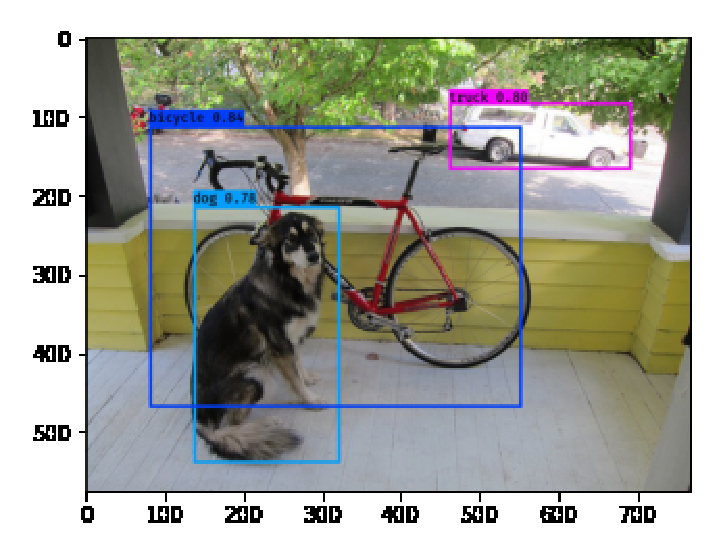
\includegraphics{output_29_1}
    \end{center}
    { \hspace*{\fill} \\}
    
    \begin{center}
    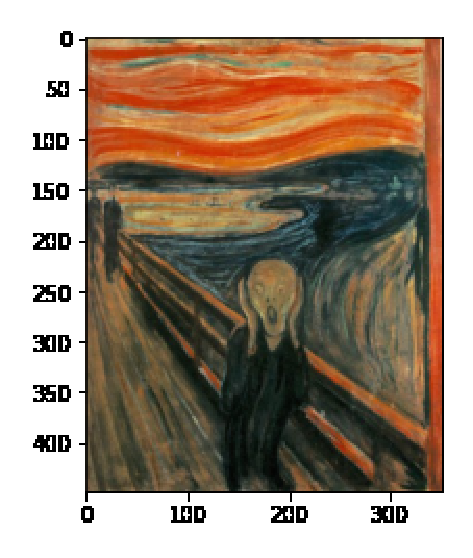
\includegraphics{output_29_2}
    \end{center}
    { \hspace*{\fill} \\}
    
    \begin{center}
    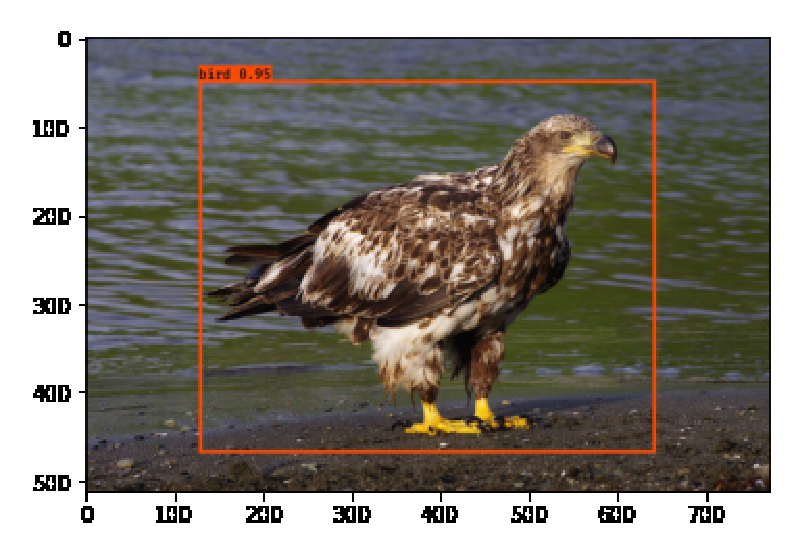
\includegraphics{output_29_3}
    \end{center}
    { \hspace*{\fill} \\}
    
    \begin{center}
    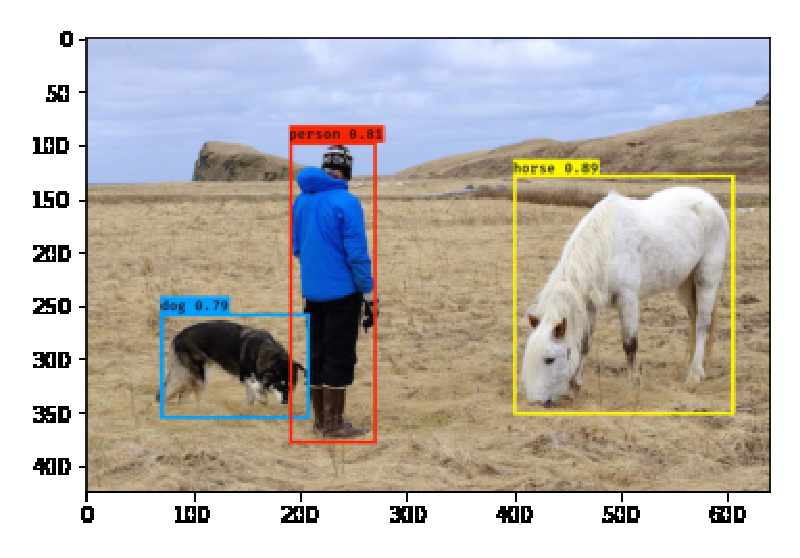
\includegraphics{output_29_4}
    \end{center}
    { \hspace*{\fill} \\}
    
    \begin{center}
    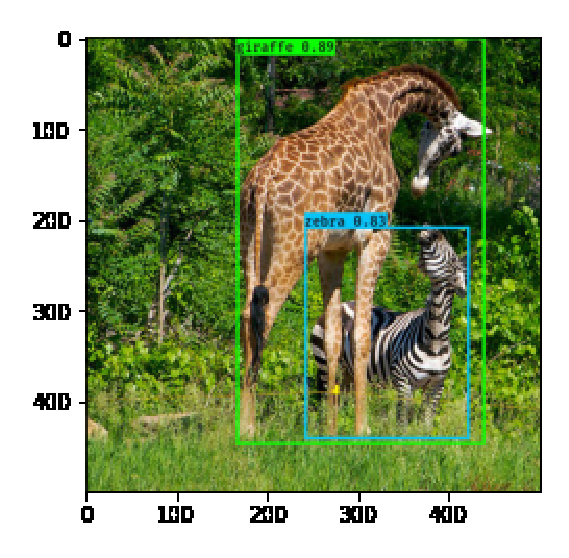
\includegraphics{output_29_5}
    \end{center}
    { \hspace*{\fill} \\}
    
    \begin{center}
    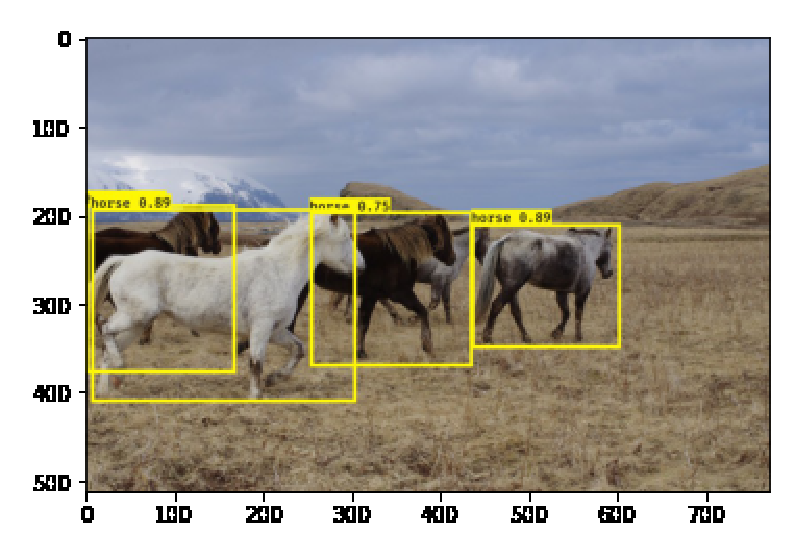
\includegraphics{output_29_6}
    \end{center}
    { \hspace*{\fill} \\}
    
    \begin{tcolorbox}[breakable, size=fbox, boxrule=1pt, pad at break*=1mm,colback=cellbackground, colframe=cellborder]
\prompt{In}{incolor}{23}{\boxspacing}
\begin{Verbatim}[commandchars=\\\{\}]
\PY{k}{for} \PY{n}{filename} \PY{o+ow}{in} \PY{n}{os}\PY{o}{.}\PY{n}{listdir}\PY{p}{(}\PY{l+s+s1}{\PYZsq{}}\PY{l+s+s1}{./images}\PY{l+s+s1}{\PYZsq{}}\PY{p}{)}\PY{p}{:}
    \PY{k}{if} \PY{n}{filename}\PY{o}{.}\PY{n}{endswith}\PY{p}{(}\PY{l+s+s1}{\PYZsq{}}\PY{l+s+s1}{.jpg}\PY{l+s+s1}{\PYZsq{}}\PY{p}{)}\PY{p}{:}
        \PY{n}{predict}\PY{p}{(}\PY{n}{sess}\PY{p}{,} \PY{l+s+s1}{\PYZsq{}}\PY{l+s+s1}{./images/}\PY{l+s+s1}{\PYZsq{}} \PY{o}{+} \PY{n+nb}{str}\PY{p}{(}\PY{n}{filename}\PY{p}{)}\PY{p}{)}
\end{Verbatim}
\end{tcolorbox}

    \begin{center}
    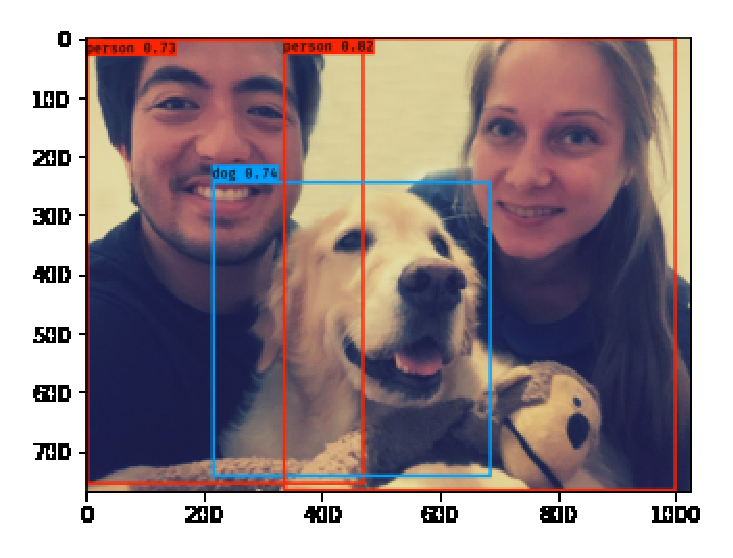
\includegraphics{output_30_0}
    \end{center}
    { \hspace*{\fill} \\}
    
    \begin{center}
    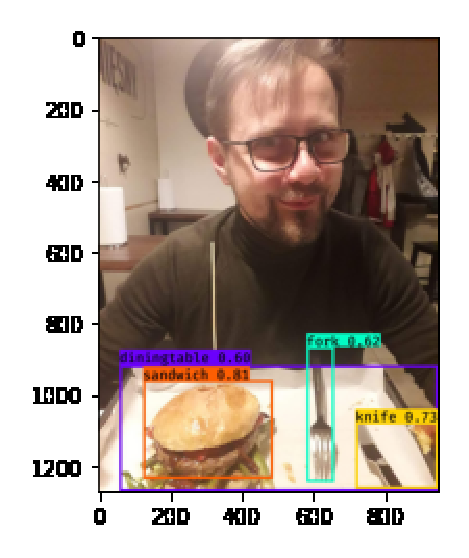
\includegraphics{output_30_1}
    \end{center}
    { \hspace*{\fill} \\}
    
    \begin{center}
    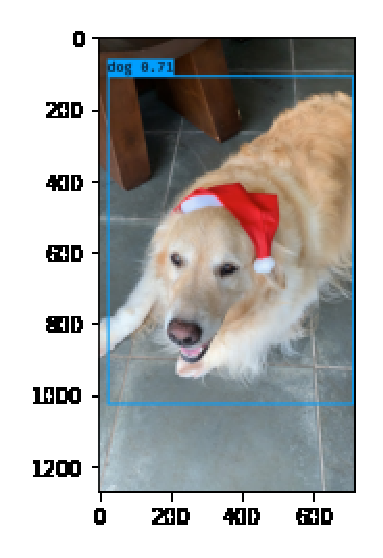
\includegraphics{output_30_2}
    \end{center}
    { \hspace*{\fill} \\}
    
    \begin{center}
    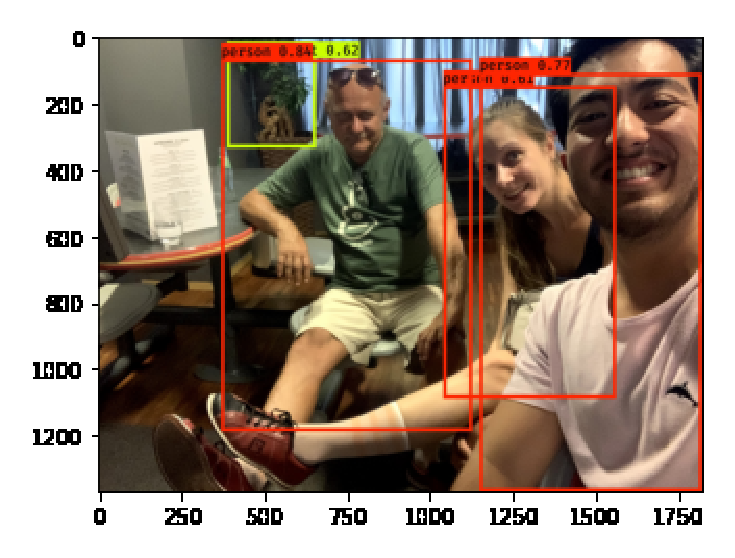
\includegraphics{output_30_3}
    \end{center}
    { \hspace*{\fill} \\}
    
    \begin{tcolorbox}[breakable, size=fbox, boxrule=1pt, pad at break*=1mm,colback=cellbackground, colframe=cellborder]
\prompt{In}{incolor}{ }{\boxspacing}
\begin{Verbatim}[commandchars=\\\{\}]

\end{Verbatim}
\end{tcolorbox}


    % Add a bibliography block to the postdoc
    
    
    
\end{document}
